\section{Informationsdarstellung}
\subsection{Begriffe und Definitionen}

\begin{minipage}[t]{9cm}
	\subsubsection{Maschinenwort}
	Das Maschinenwort ist die endliche geordnete Folge von Bin"arzeichen, die im Computer als Einheit verarbeitet werden kann. Es entspricht der Gr"osse des Rechenwerks und wird auch \dq Word\dq \ \ genannt.
	
	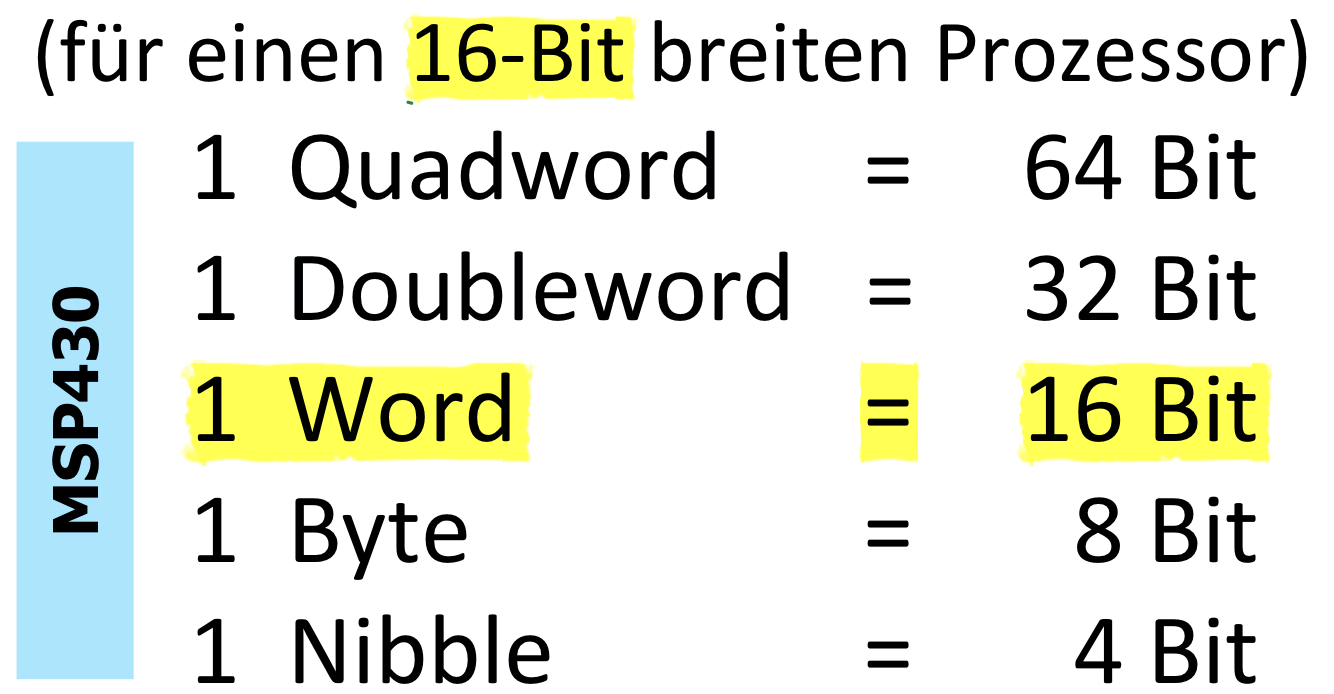
\includegraphics[width = 5cm]{pics/Wortlaenge}

	\subsubsection{Informationsparameter (Signal Parameter)}
	Die Kenngr"osse eines Signals, dessen Wert die Information beinhaltet.
	Bie einer Wechselspannung w"are das zum Beispiel die Amplitude, die Frequenz oder der Phasenwinkel.

\end{minipage}
%
\begin{minipage}{0.5cm}
	\ \
\end{minipage}
%
\begin{minipage}[t]{9cm}
	\subsubsection{Signalarten}
	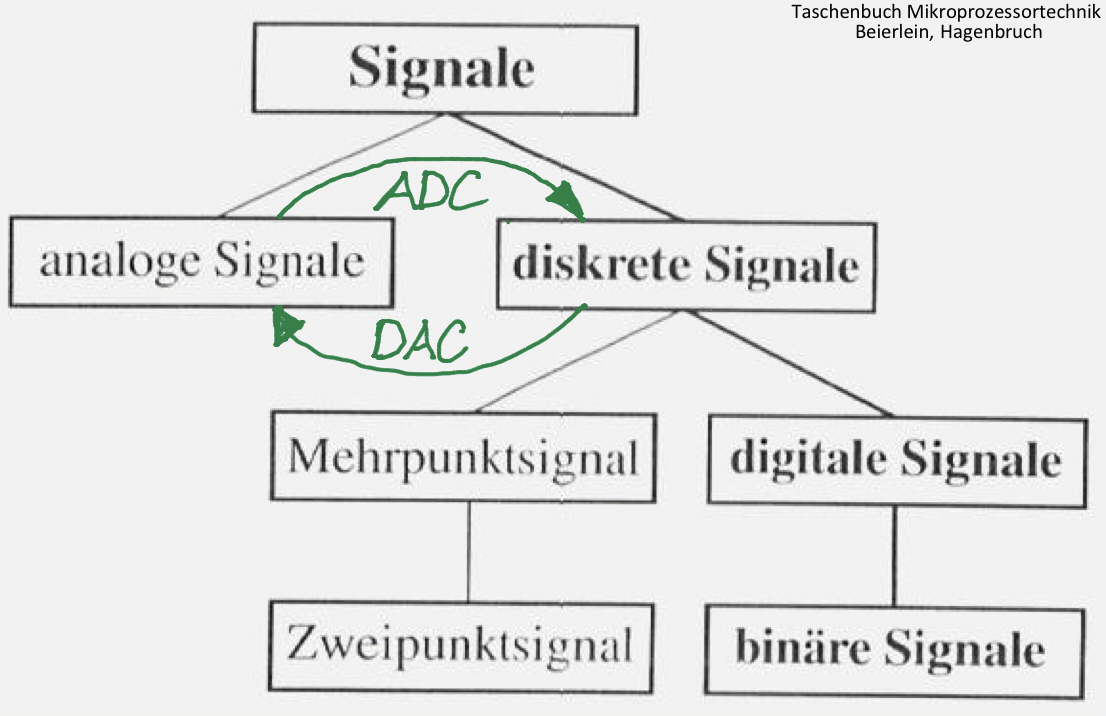
\includegraphics[width=8cm]{pics/Signalarten}
\end{minipage}

\begin{minipage}[t]{9cm}
\ \
	\subsection{Grundlegende Datenarten}
	Sowohl auf der Input- wie auch auf der Output-Seite werden drei verschiedene, grundlegende Datenarten unterschieden:
	
	\textbf{Signale}, welche beim Auftreten eines Ereignisses Information liefern, sind Zeitlich zuf"allig

	\textbf{Daten-Meldungen} liefern Daten, welche Informationen enthalten, auch zu einem zuf"alligen Zeitpunkt.

	\textbf{Datenstr"ome} m"ussen periodisch abgetastet, "ubertragen und in der gleichen sequenziellen Reihenfolge verarbeitet werden.
	
	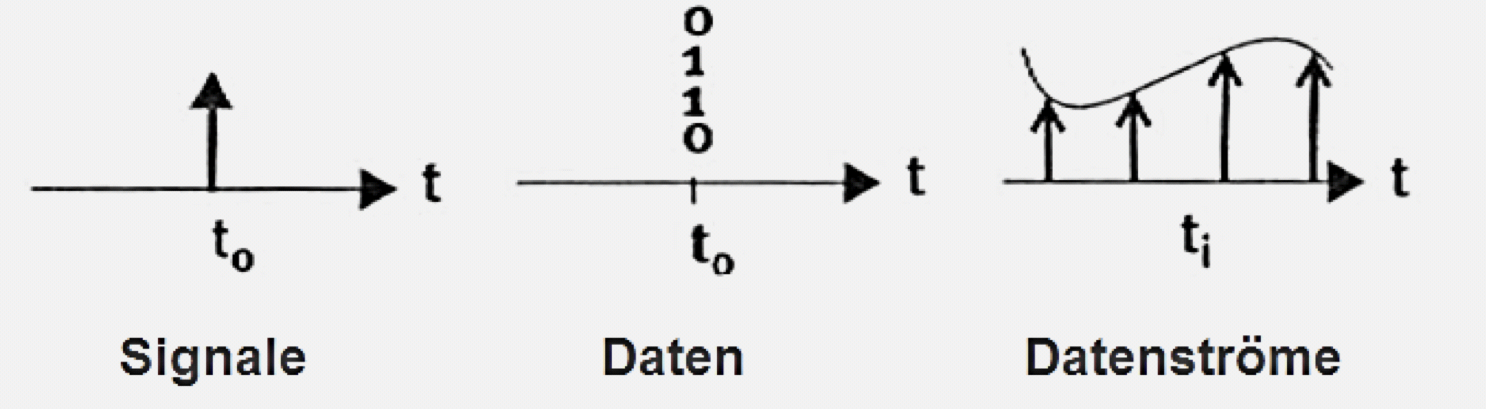
\includegraphics[width=6cm]{pics/Datenarten}
	
	\subsection{Gr"ossen-Angaben bei Speichern}
	Auf das Bin"arsystem bezogen werden die Bezeichnungen Kilo(K), Mega(M) und Giga (G) verwendet, damit es keine Verwechslung gibt, denn: \textbf{1K $\neq$ 1k = $10^3$}

	\textbf{1K} = $2^{10}$ = 1024\\
	\textbf{1M} = 1024K = 1048576\\
	\textbf{1G} = 1024M
	\end{minipage}
%
\begin{minipage}{0.5cm}
	\ \
\end{minipage}
%
\begin{minipage}[t]{9cm}
\ \
	\subsection{ASCII-Code}
	Die Kodierung eines Zeichen setzt sich aus sieben Bits zusammen. Neben Zeichen gibt es auch noch Steuerfunktionen. Die Kodierung eines Zeichens setzt sich folglich zusammen: \dq 0x Spaltenindex Zeilenindex\dq  (z.B. \dq V\dq = 0x56)
	
	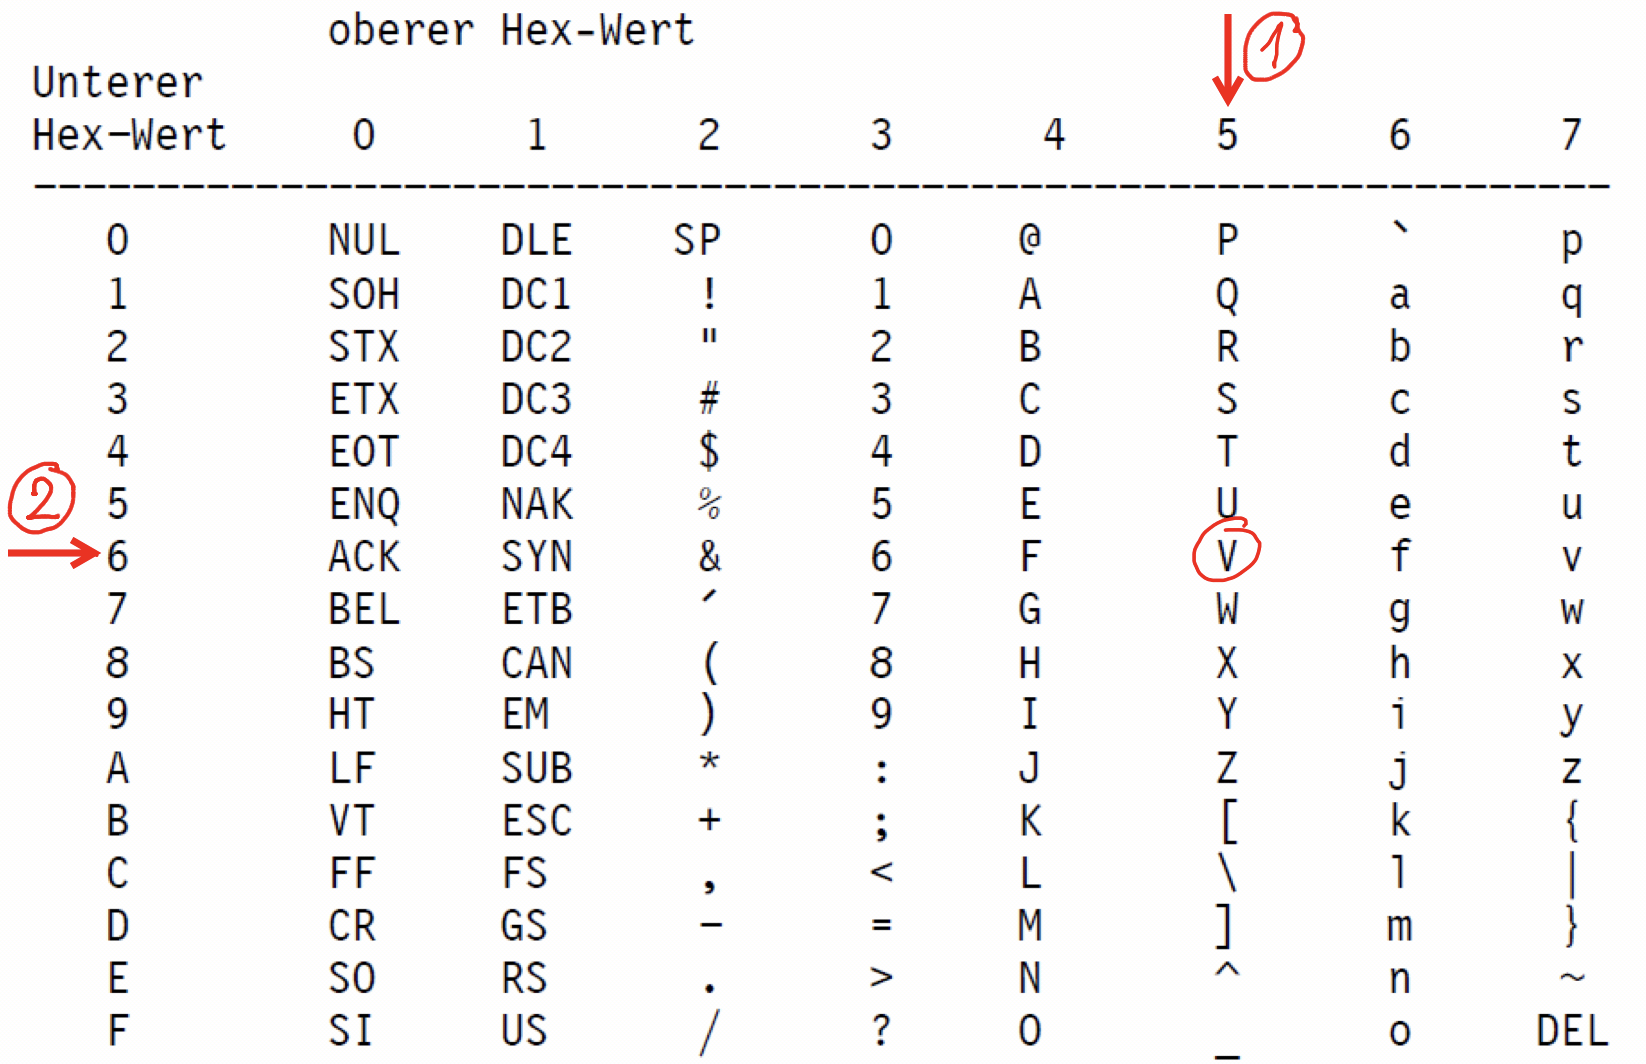
\includegraphics[width=9cm]{pics/ASCII-Tabelle}
\end{minipage}

\subsection{Zahlensysteme}
Zwischen dem Dezimal-, Bin"ar-, Oktal- und Hexadezimalsystem k"onne die Zahlen relativ einfach umgerechnet werden. Eine Zahl im \textbf{Bin"arsystem} wird \textbf{\%} gekennzeichnet, eine Zahl im \textbf{Oktalsystem} mit \textbf{@} und eine Zahl im \textbf{Hexadezimalsystem} mit \textbf{0x}.


\subsubsection{Umrechnung Dezimal $\Leftrightarrow$ Bin"ar $\Leftrightarrow$ Hex}
\begin{minipage}{7cm}
	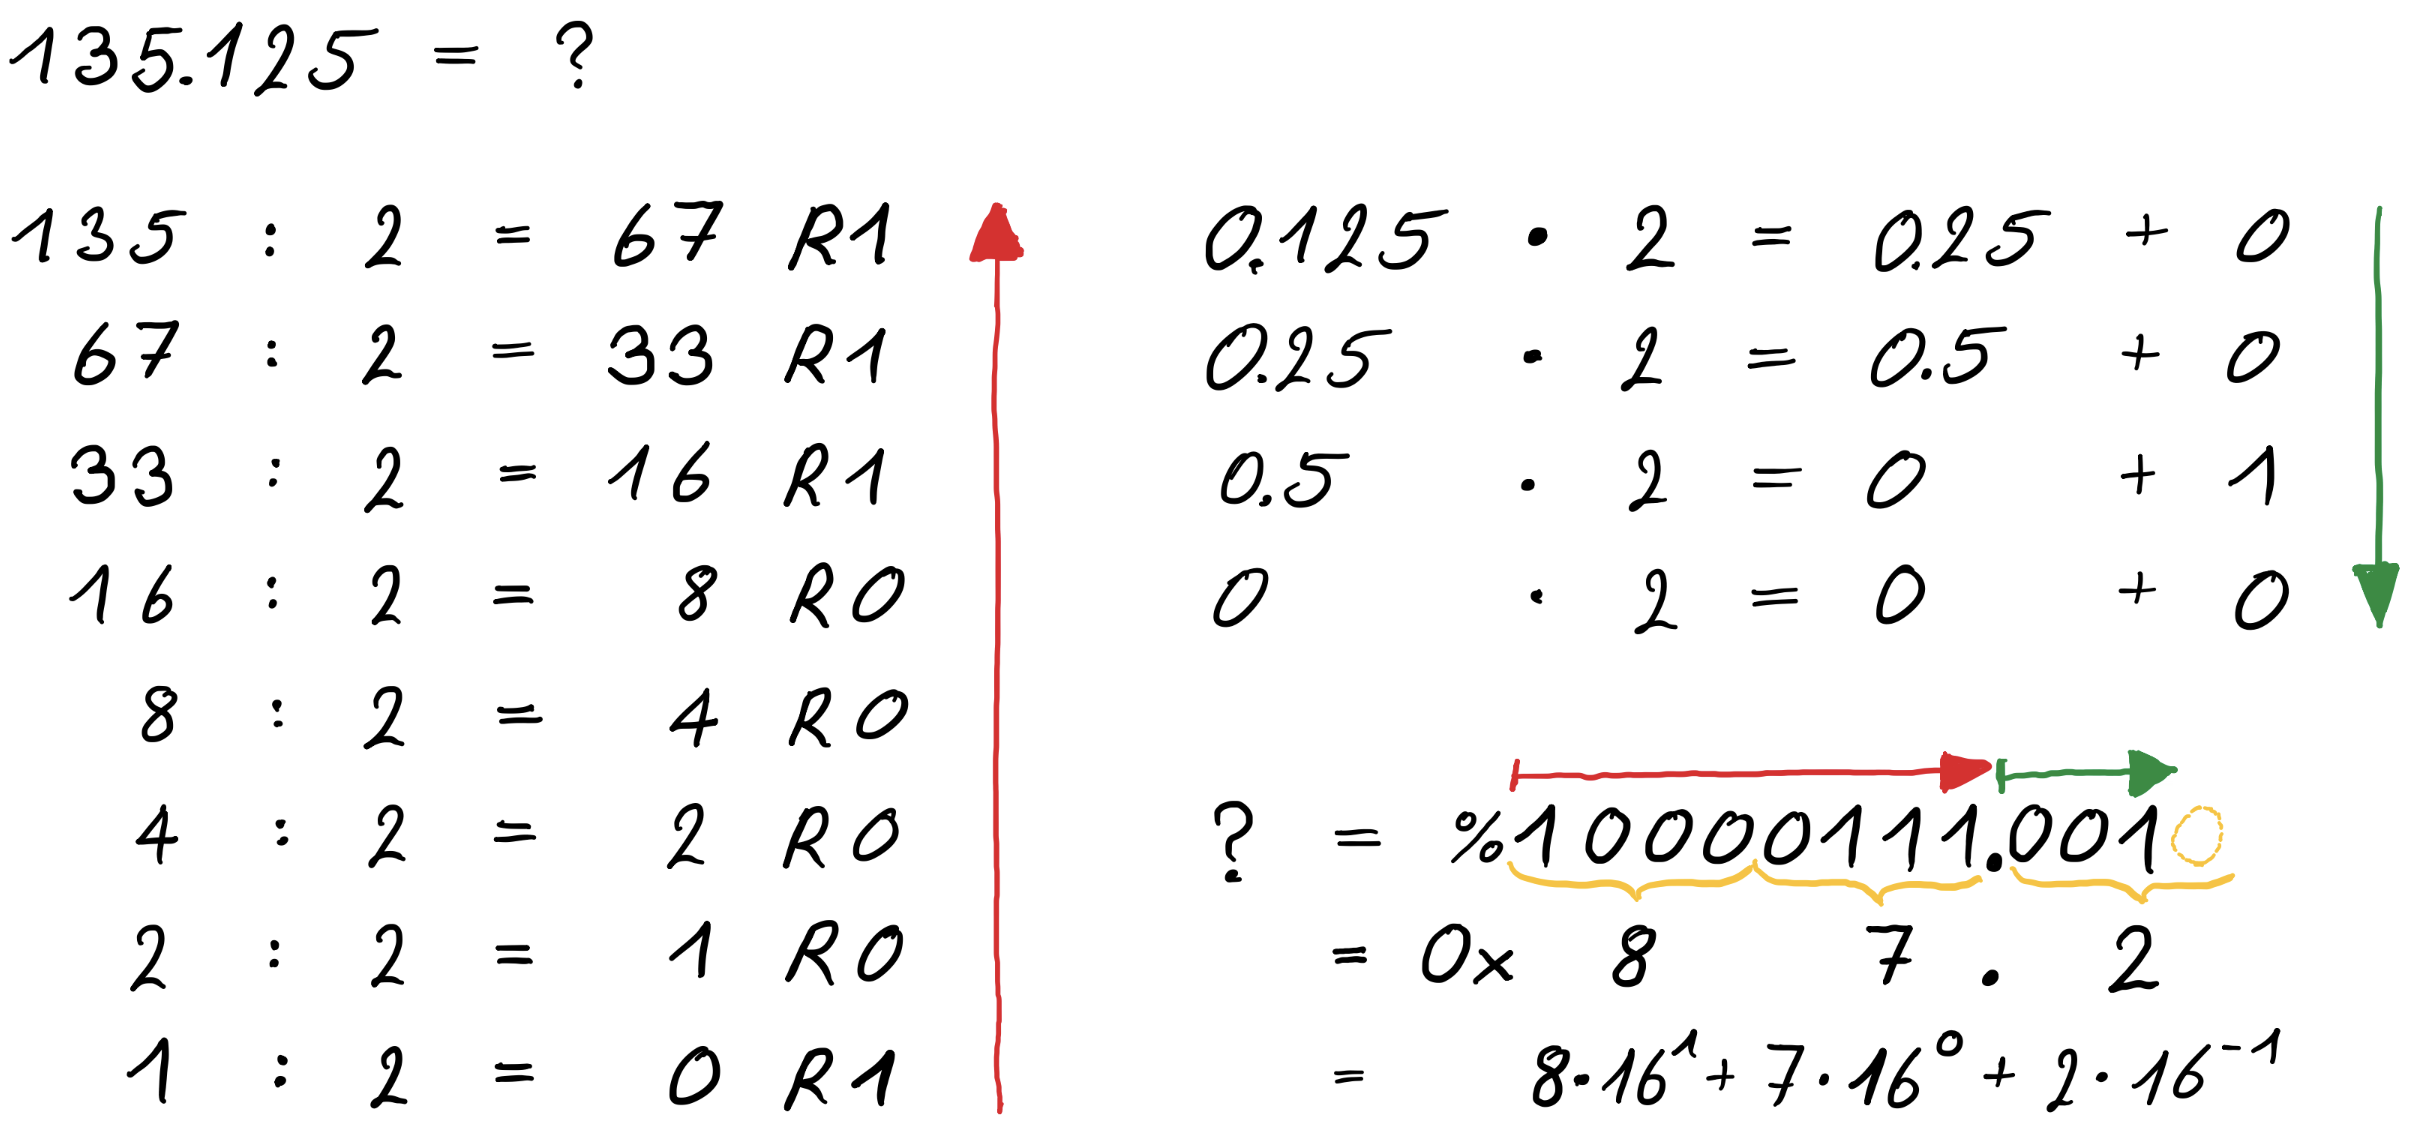
\includegraphics[width=7cm]{pics/Zahlenumrechnung}
\end{minipage}
%
\begin{minipage}{0.5cm}
	\ \
\end{minipage}
%
\begin{minipage}{11cm}
	Wenn die Bin"arzahl statt ins Hexadezimale ins \textbf{Oktalsystem} gewandelt werden soll, m"ussen statt Viererpakete Dreierpakete geb"undelt werden. 
	
	Soll eine Zahl in \textbf{BCD-Code} konvertiert werden, dann bekommt jede Ziffer der Dezimalzahl ein Nibble, mit dem Wert der Ziffer.
\end{minipage}


\begin{minipage}[t]{10cm}
	\vspace{-4ex}
	\subsubsection{Vorzeichenlose Ganzzahlen (unsigned integer)}
	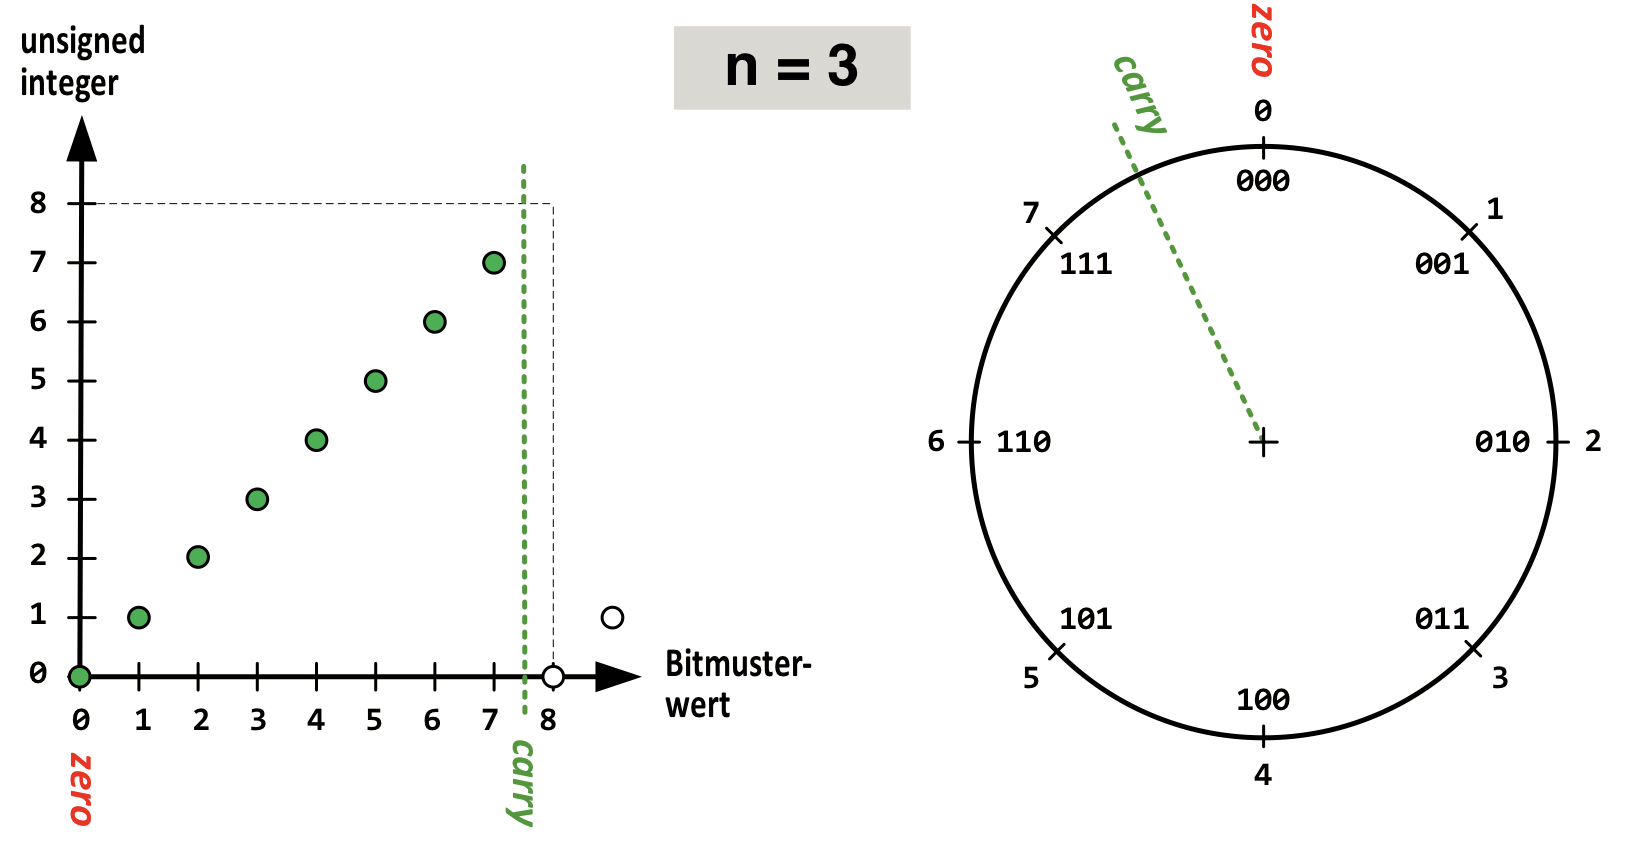
\includegraphics[width=7cm]{pics/Unsigned-Zahl}
	
	Vorzeichenlose Ganzzahlen, auch unsigned integer Zahlen gennant, k"onnen nur positive ganzzahlige Werte annehmen.
	\begin{tabbing}
		\textbf{Ca}\= \textbf{rry-Flag:}\\
		\> Wenn $a + b > 2^n -1$, dann wird das Carry-Flag gesetzt\\
		\> Wenn $a - b$ und $b > a$, dann wird auch das Carry-Flag\\
		\> gesetzt,in diesem Fall nennt man es auch \textbf{borrow}.\\

		\textbf{Zero-Flag:}\\
		\> Wenn das Resultat 0, Zero ergibt, dann wird das Zero-Flag\\ 
		\> gesetzt.
	\end{tabbing}

	\subsubsection{Zweierkomplement (signed integer)}
	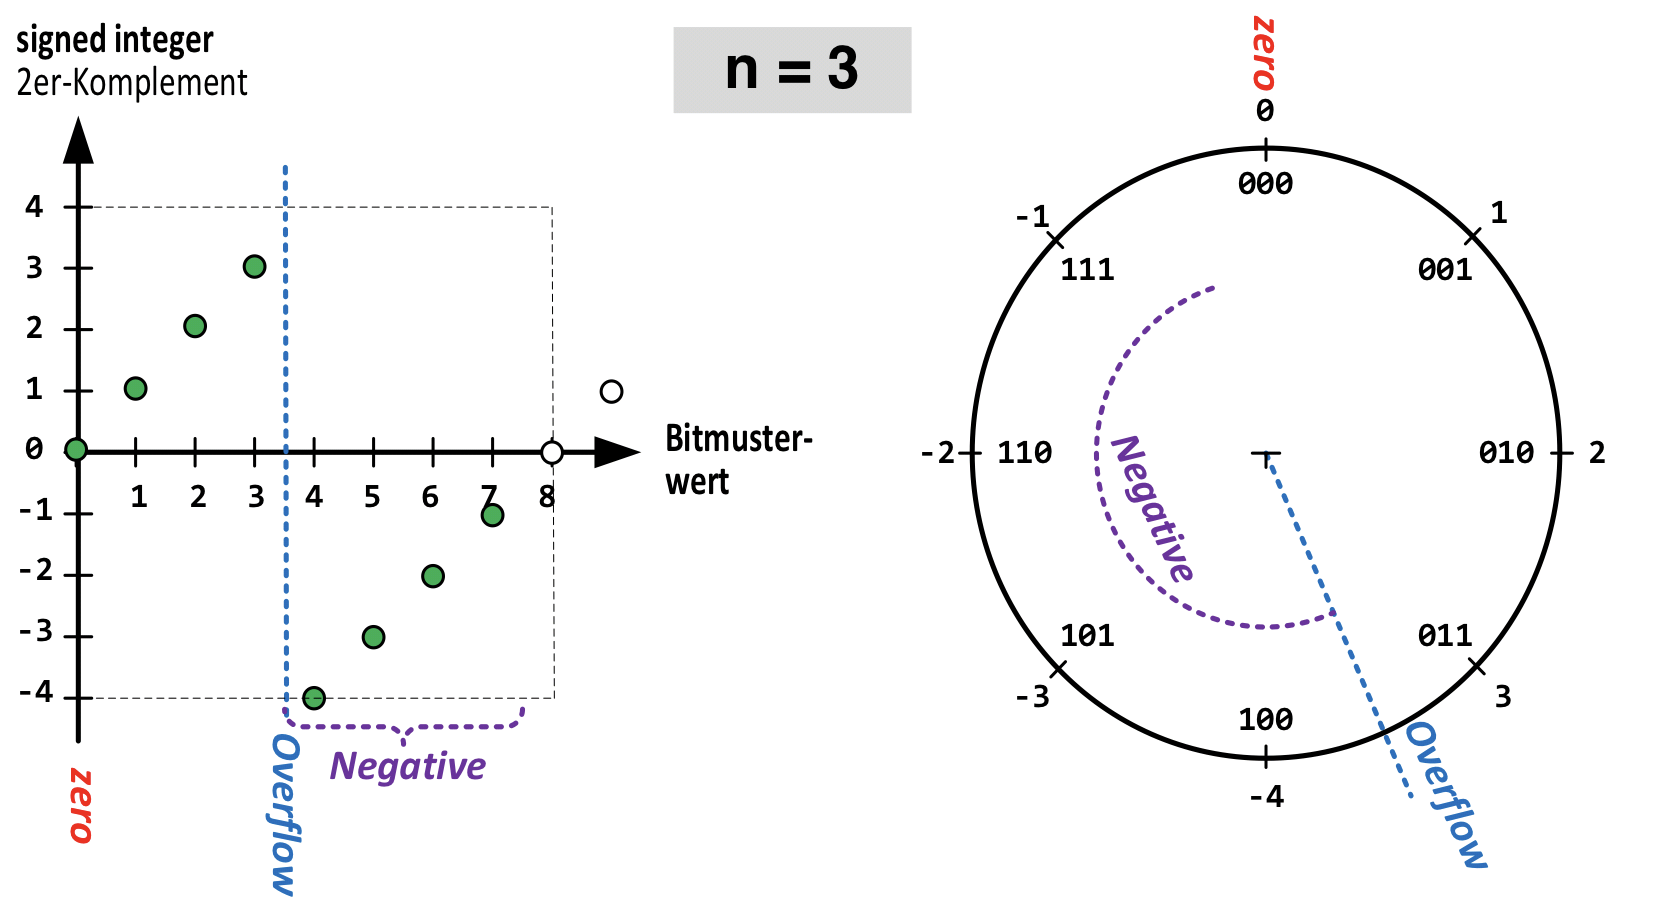
\includegraphics[width=7cm]{pics/Signed-Zahl}
	
	Vorzeichenbehaftete Ganzzahlen, auch signed integer Zahlen gennant, k"onnen positive und negative Ganzzahlwerte annehmen.
	\vspace{-2ex}
	\begin{tabbing}
		\textbf{Ne}\= \textbf{gative-Flag:}\\
		\> Wenn sich die Zahl im negativen Bereich des Zahlenkreises\\ 
		\> befindet wird das Negative-Flag gesetzt.\\

		\textbf{Overflow-Flag:}\\
		\> Wenn die Addition oder Subtraktion rein mathematisch keinen\\ 
		\> Sinn ergibt und der Overflow-Bereich auf dem Zahlenkreis\\
		\> "uberschritten wird, wird das Overflow-Flag gesetzt.
	\end{tabbing}

	\subsubsection{Duales Rechenwerk}
	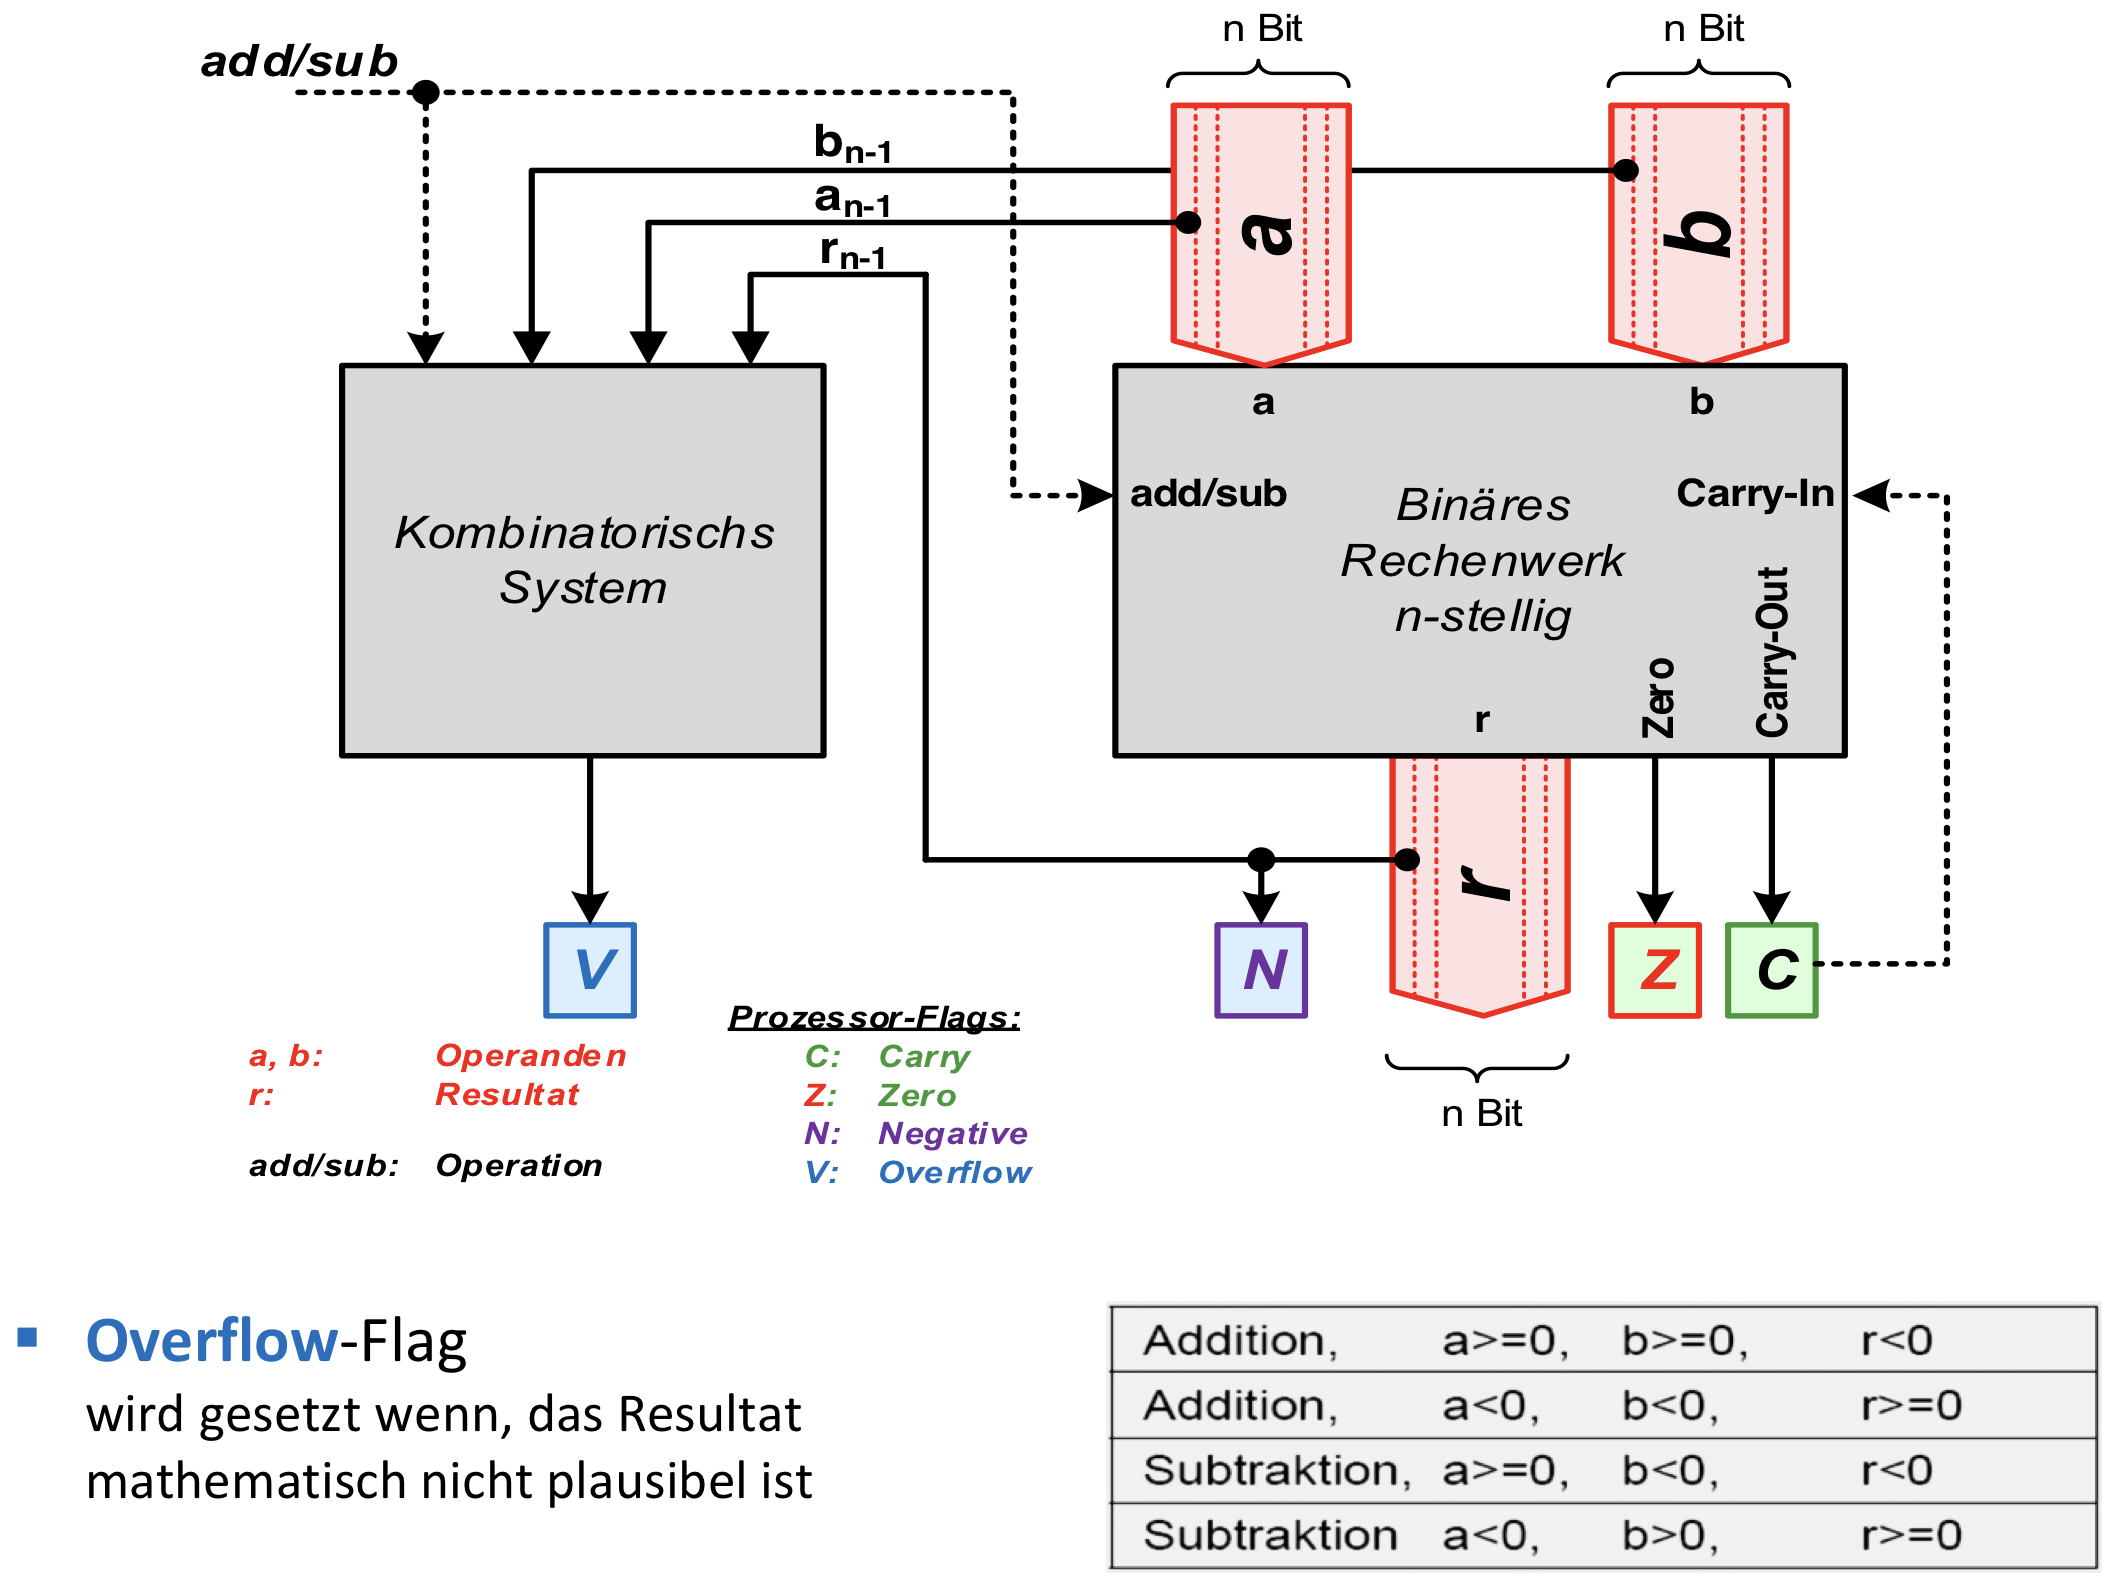
\includegraphics[width=8.5cm]{pics/Duales_rechenwerk}
	
	Das duale Rechenwerk f"uhrt nicht nur Addition und Subtraktion zweier Zahlen durch sondern setzt zudem auch das Zero- und Carry-Flag. Das Overflow-Flag muss noch mit einem kombinatorischen System bestimmt werden.
\end{minipage}
%
\begin{minipage}{0.5cm}
	\ \
\end{minipage}
%
\begin{minipage}[t]{8cm}
	\vspace{-4ex}
	\subsubsection{Operationen im dualen Rechenwerk}
	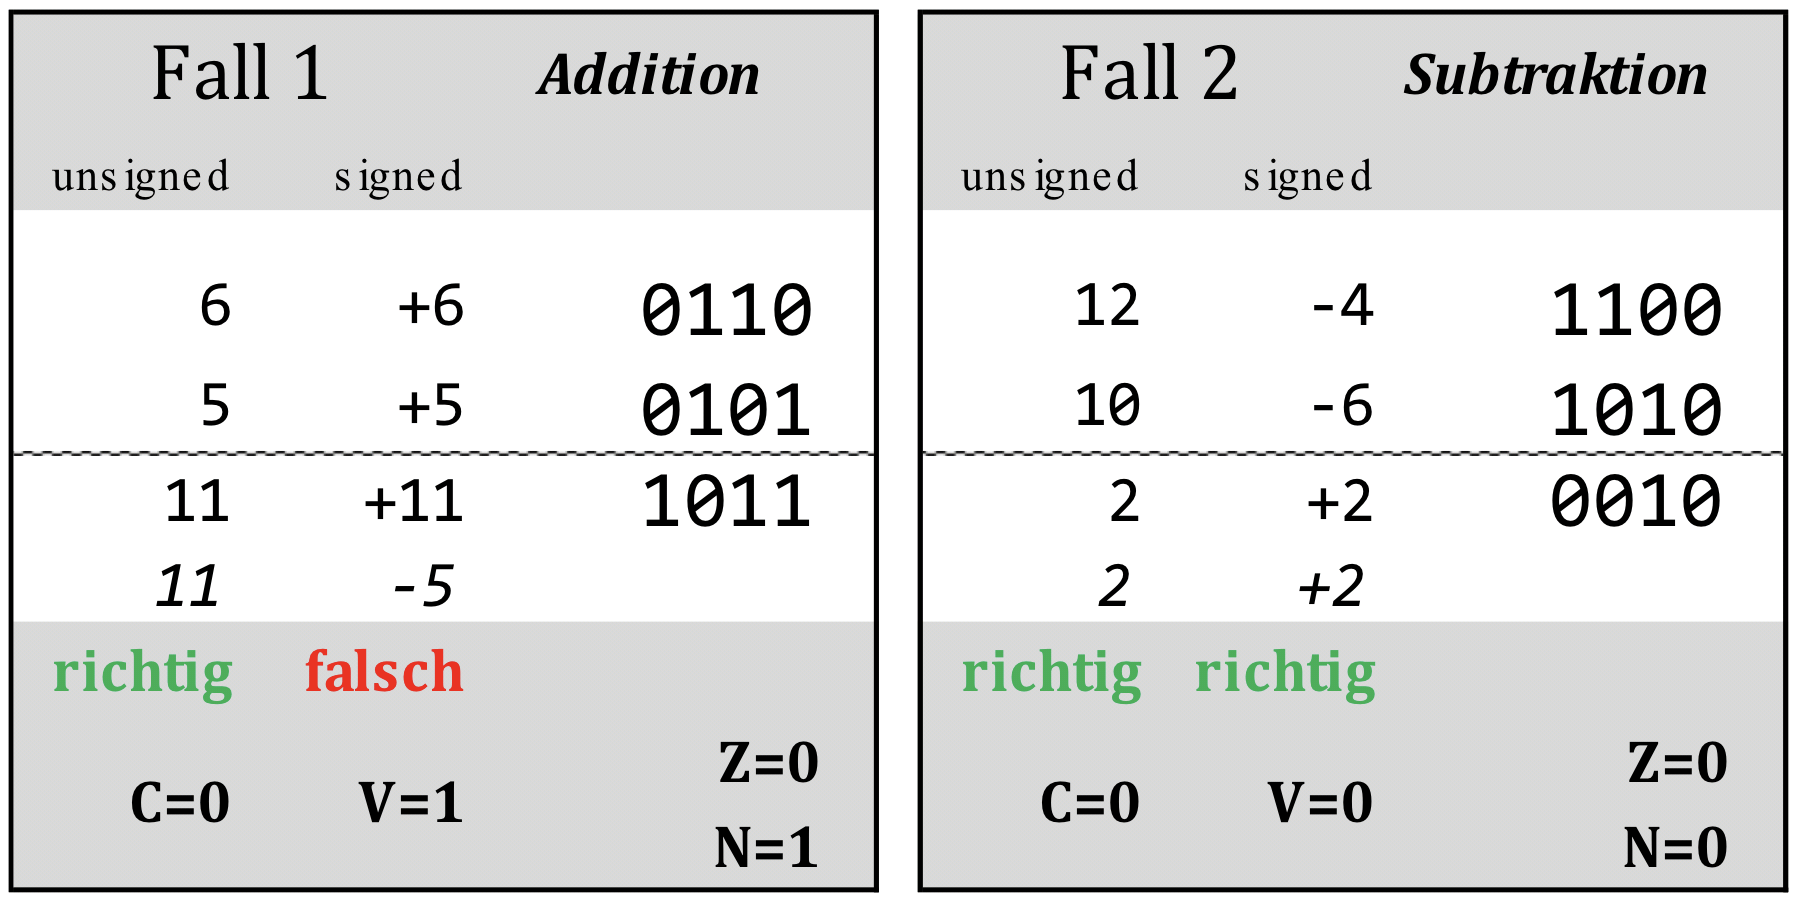
\includegraphics[width = 8cm]{pics/Bsp-Zahlenkreis-Zahlen}
	
	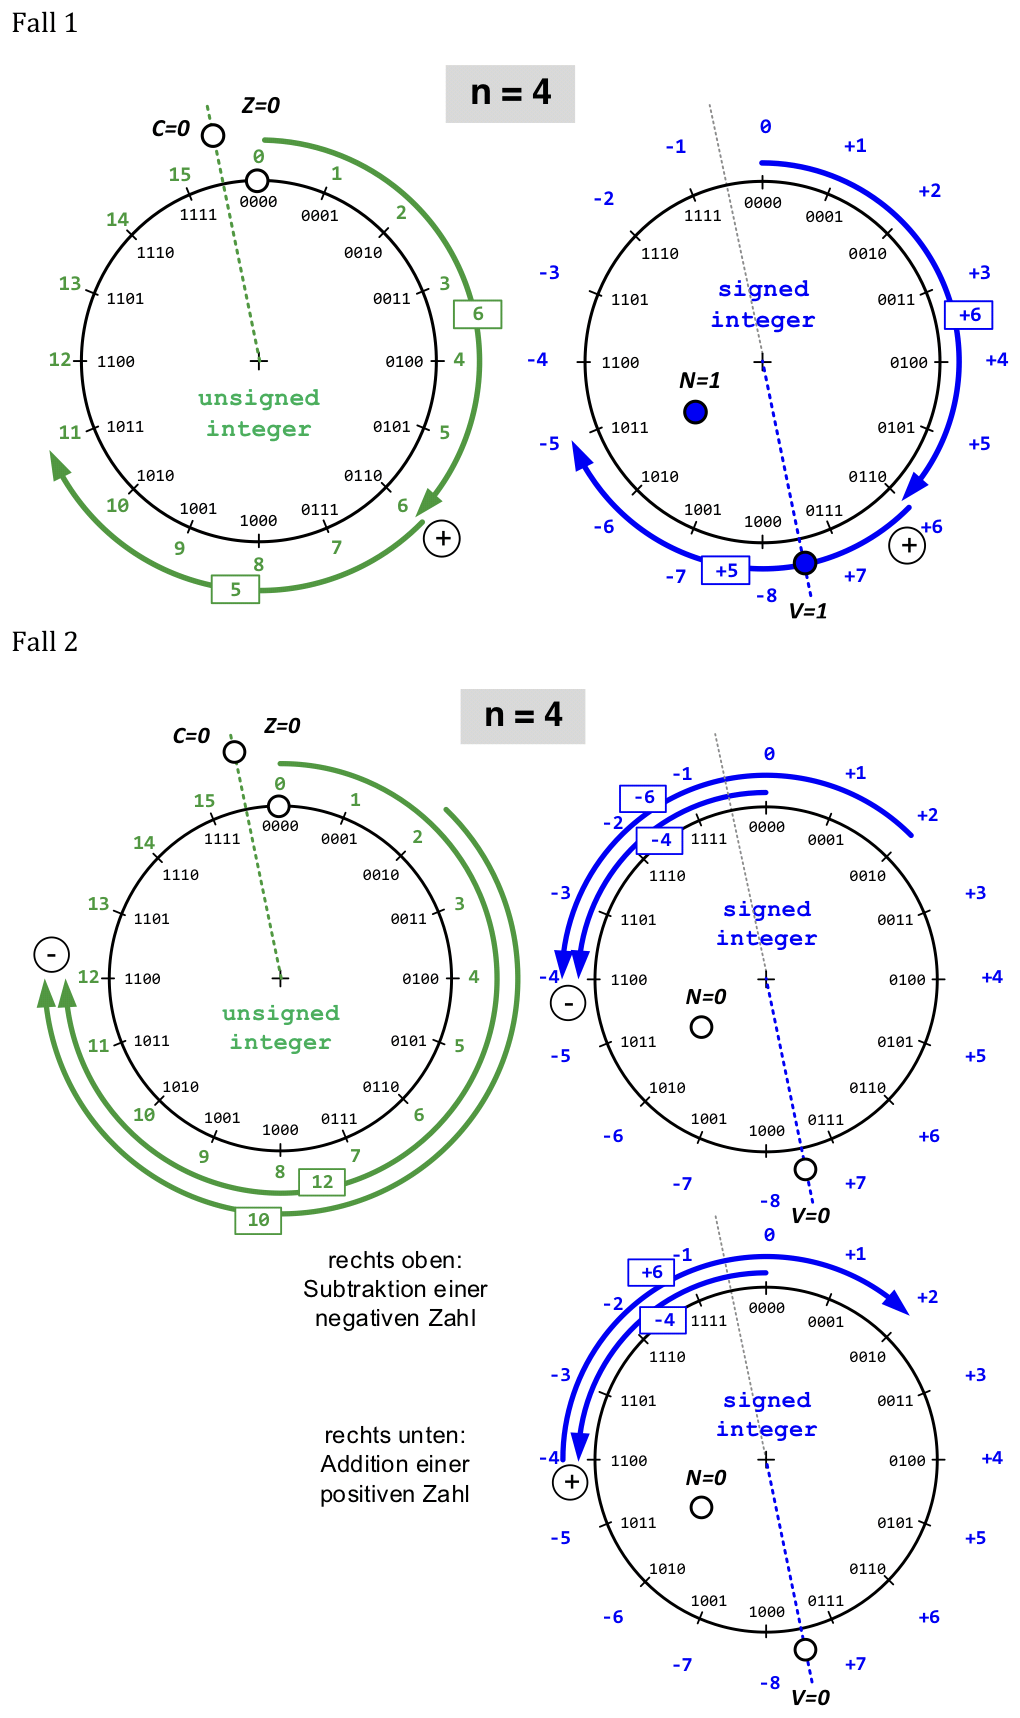
\includegraphics[width = 8cm]{pics/Bsp-Zahlenkreis}
	\begin{tabbing}
		\textbf{Al}\= \textbf{lgemeine Zahlenkreis Regeln}\\
		\> Addition: Zahlenvektoren hintereinander reihen\\
		\> Subtraktion: Zahlenvektoren stumpf gegeneinander\\
		\> stellen\\

		\textbf{signed integer}\\
		\> Flags: Negative, Overflow, Zero\\
		\> positiv: Zahlenvektoren Uhrzeigersinn\\
		\> negativ: Zahlenvektoren Gegenuhrzeigersinn\\
	
		\textbf{unsigned integer}\\
		\> Flags: Zero, Carry\\
		\> Zahlenvektoren immer Uhrzeigersinn\\
	\end{tabbing}
\end{minipage}

\subsection{Alternative Darstellungen von vorzeichenbehafteten Ganzzahlen}
\subsubsection{Gr"ossendarstellung mit Vorzeichen (signed magnitude)}
\vspace{-2ex}
\begin{minipage}{9cm}
	\begin{tabbing}
		MS\=B gibt  Vorzeichen an:\\
		\> $d_{n-1} = 0 \Rightarrow$ positive Zahl\\
		\> $d_{n-1} = 1 \Rightarrow$ negative Zahl\\\\
		
		Bemerkungen, Probleme:\\
		\> Es entstehen zwei verschiedene Darstellungen der Null\\
		\> z.B. bei n = 8: \= +0 \= = \%00000000\\
						\> \> -0 \> = \%10000000
		
	\end{tabbing}
\end{minipage}
%
\begin{minipage}{0.5cm}
	\ \
\end{minipage}
%
\begin{minipage}{9cm}
	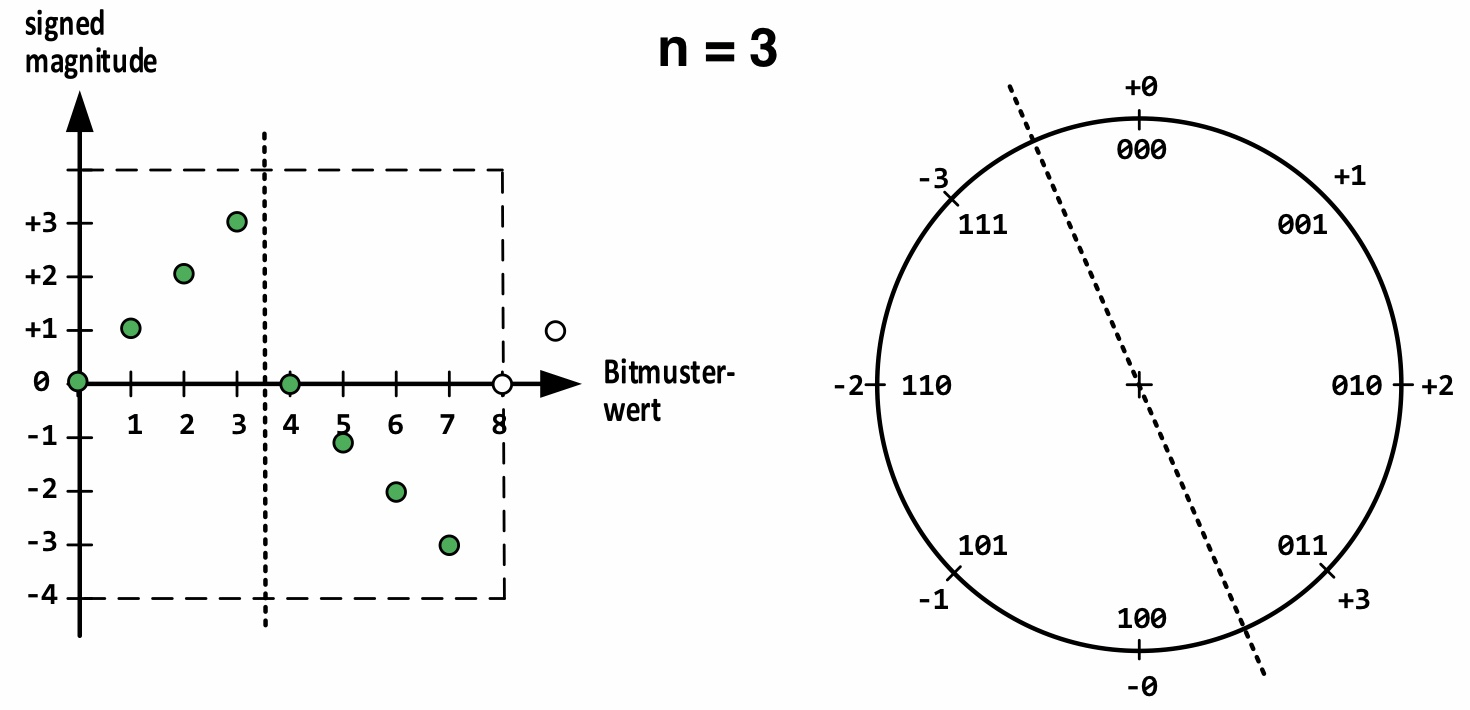
\includegraphics[width=8cm]{pics/Signed_Magnitude}
\end{minipage}

\subsubsection{Einerkomplement}
\vspace{-2ex}
\begin{minipage}{9cm}
	\begin{tabbing}
		MS\=B gibt  Vorzeichen an:\\
		\> $d_{n-1} = 0 \Rightarrow$ positive Zahl\\
		\> $d_{n-1} = 1 \Rightarrow$ negative Zahl\\\\
		
		Bemerkungen, Probleme:\\
		\> Es entstehen zwei verschiedene Darstellungen der Null\\
		\> z.B. bei n = 8: \= +0 \= = \%00000000\\
						\> \> -0 \> = \%11111111
		
	\end{tabbing}
\end{minipage}
%
\begin{minipage}{0.5cm}
	\ \
\end{minipage}
%
\begin{minipage}{9cm}
	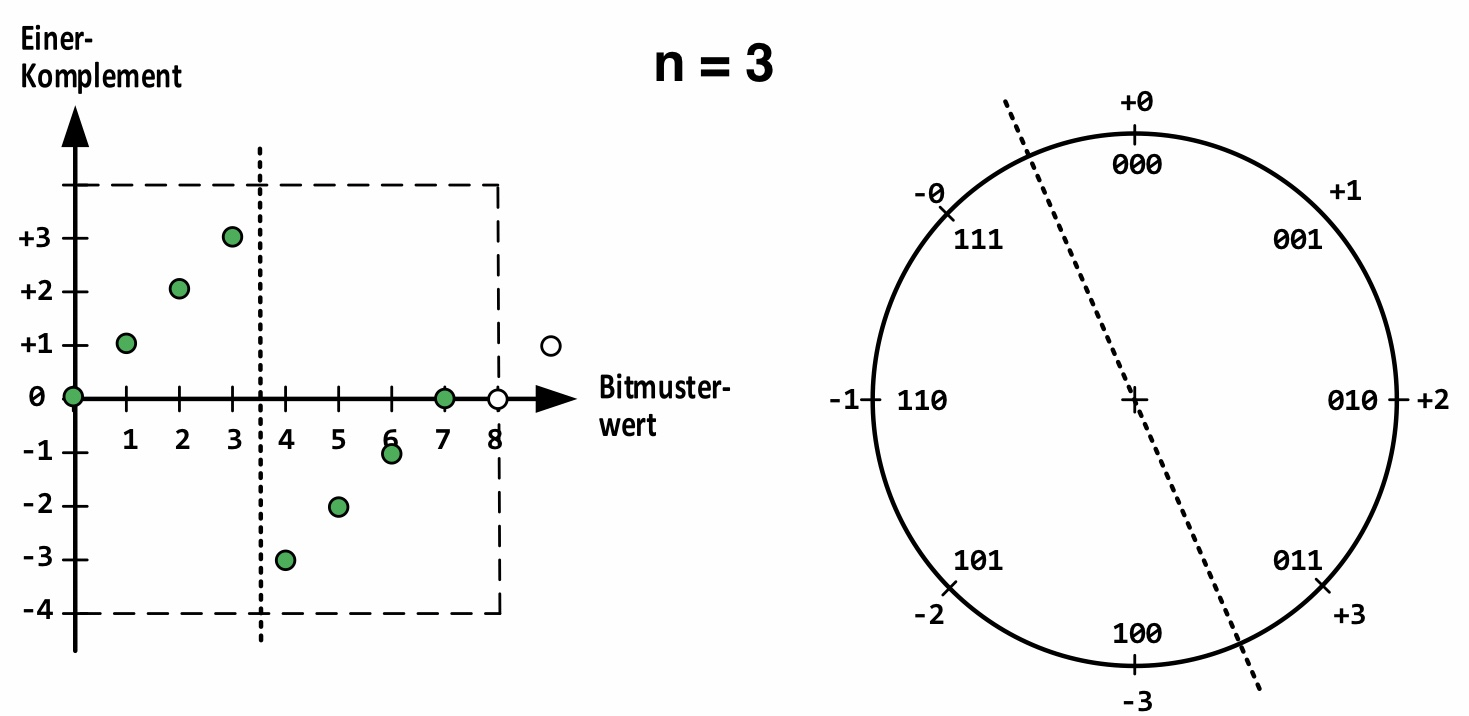
\includegraphics[width=8cm]{pics/Ones_Complement}
\end{minipage}

\subsubsection{Excess-Code, Stibitz-Code}
\begin{minipage}{9cm}
	\begin{tabbing}
		MS\=B gibt  Vorzeichen an:\\
		\> $d_{n-1} = 1 \Rightarrow$ positive Zahl\\
		\> $d_{n-1} = 0 \Rightarrow$ negative Zahl\\
		Wert = Bitmusterwert - $2^{n-1}$\\\\
		Bemerkungen, Probleme:\\
		\> Eindeutiges Bitmuster f"ur Null\\
		\> Zweierkomplement um den Exzess von $\mathbf{2^{n-1}}$ verschoben\\
		\> Excess-Code wird beispielsweise f"ur die Floating-Point \\
		\> Darstellung verwendet	
	\end{tabbing}
\end{minipage}
%
\begin{minipage}{0.5cm}
	\ \
\end{minipage}
%
\begin{minipage}{9cm}
	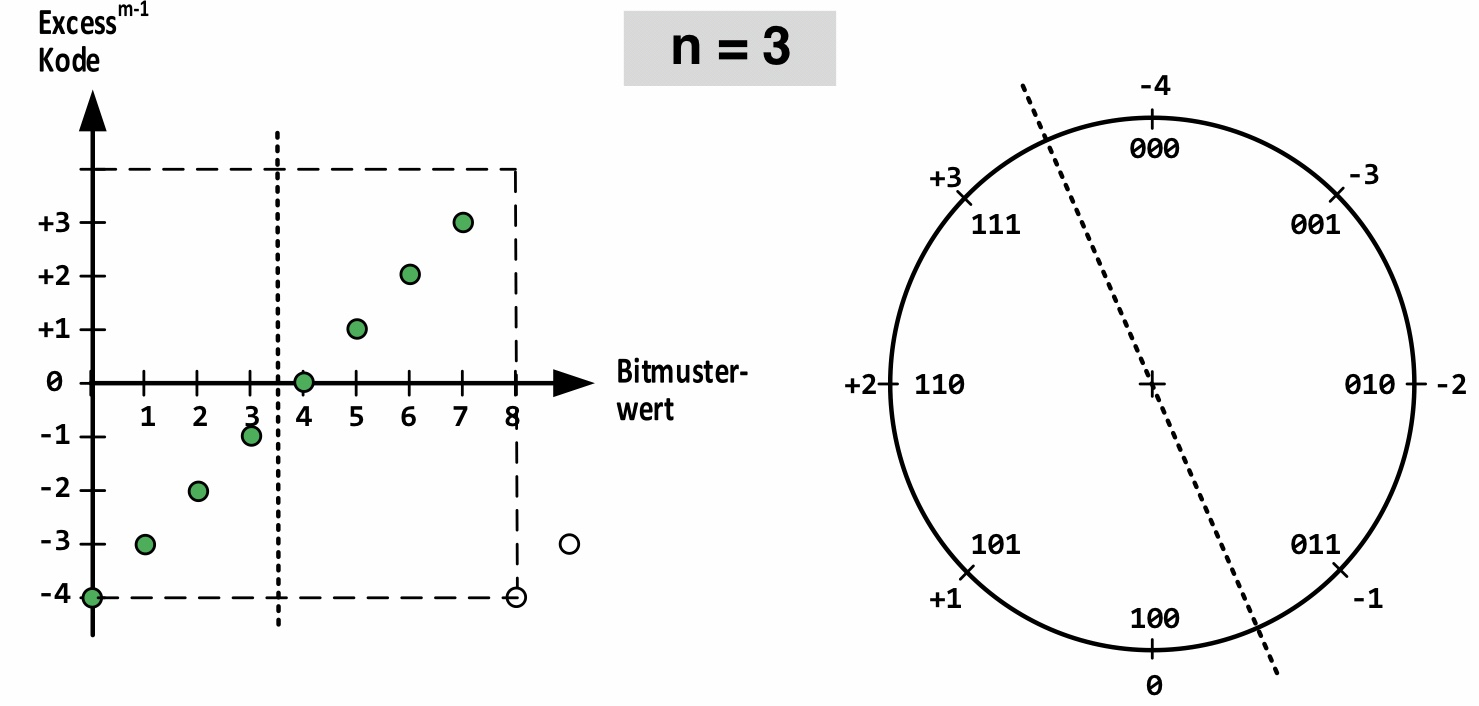
\includegraphics[width=8cm]{pics/Excess_Code}
\end{minipage}

\subsection{Festkommazahlen}
\begin{minipage}[t]{9cm}
	\subsubsection{IQ-Zahlen Format}
	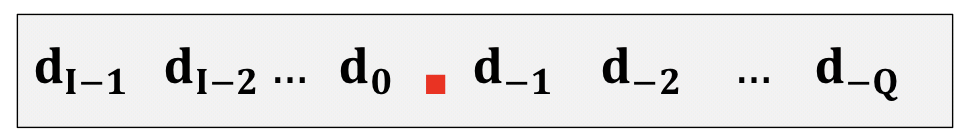
\includegraphics[width=5cm]{pics/IQ-Zahlen}
	\begin{itemize}
		\item \textbf{I}: Anzahl Integer-Stellen (Vorkommabitanzahl)
		\item \textbf{Q}: Anzahl Quotient-Stellen (Nachkommabitanzahl)
		\item Optimales Verh"altnis zwischen der erforderlichen Genauigkeit und dem n"otigen Wertebereich der Zahlendarstellung.
		\item Trennpunkt ist nur unsere Interpretation, Festkomma-Rechner rechnen immer mit reinen Bin"arzahlen
		\item Multiplikation und Division mit 2 kann mit Neuinterpretation der Bitfolge erreicht werden. \\(z.B. /2: I3Q2 $\Rightarrow$ I2Q3)
		\item \begin{tabular}{|l|l|l|l|}
				\hline
				\rowcolor[HTML]{C0C0C0} 
				Format             & Bin"ar          & Dezimal                       & Genauigkeit                \\ \hline
				\rowcolor[HTML]{EFEFEF} 
				{\color[HTML]{000000} I1Q3} & {\color[HTML]{000000} 1.000 ... 0.111} & {\color[HTML]{000000} -1 ... +7/8}  & {\color[HTML]{000000} 1/8} \\ \hline
				\rowcolor[HTML]{EFEFEF} 
				{\color[HTML]{000000} I2Q2} & {\color[HTML]{000000} 10.00 ... 01.11} & 	{\color[HTML]{000000} -2 ... +1.75} & {\color[HTML]{000000} 1/4} \\ \hline
				\rowcolor[HTML]{EFEFEF} 
				{\color[HTML]{000000} I3Q1} & {\color[HTML]{000000} 100.0 ... 011.1} & {\color[HTML]{000000} -4 ... +3.5}  & {\color[HTML]{000000} 1/2} \\ \hline
				\rowcolor[HTML]{EFEFEF} 
				{\color[HTML]{000000} I4Q0} & {\color[HTML]{000000} 1000 ... 0111}   & {\color[HTML]{000000} -8 ... +7}    & {\color[HTML]{000000} 1}   \\ \hline
			\end{tabular}	
	\end{itemize}
\end{minipage}
%
\begin{minipage}{0.5cm}
	\ \
\end{minipage}
%
\begin{minipage}[t]{9cm}
	\subsubsection{Fraktionale Zahlen}
		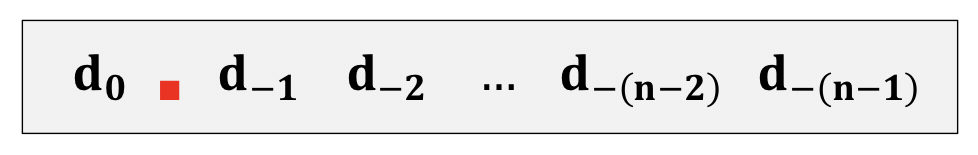
\includegraphics[width=5cm]{pics/Fraktionale_Zahlen}
		\begin{itemize}
			\item $\mathbf{d_0}$ gibt das Vorzeichen an
			\item Der Wertebereich ist immer: \color{blue} $\mathbf{-1.0 \leq W < +1.0}$ \color{black}
			\item Die Genauigkeit h"angt von der Bitanzahl \textbf{n} ab 
				\\$\Rightarrow$ \color{blue} $\mathbf{2^{-(n-1)}}$ \color{black}
			\item Wird h"aufig als Relativzahl oder Per-Unit-Zahl (PU) bezeichnet, da man den Wert prozentual zwischen $-100\%$ und $<+100\%$ auffassen kann.
			\item \begin{tabular}{|l|l|l|}
					\hline
					\rowcolor[HTML]{C0C0C0} 
					Bitanzahl & Dezimaler Wertebereich         & Schrittweite                  \\ \hline
					\rowcolor[HTML]{EFEFEF} 
					4         & $-1 \leq W <+1$ & $2^{-3}$     \\ \hline
					\rowcolor[HTML]{EFEFEF} 
					16        & $-1 \leq W <+1$ & $2^{-15}$    \\ \hline
					\rowcolor[HTML]{EFEFEF} 
					32        & $-1 \leq W <+1$ & $2^{-31}$ \\ \hline
					\rowcolor[HTML]{EFEFEF} 
					n         & $-1 \leq W <+1$ & $2^{-(n-1)}$ \\ \hline		
				\end{tabular}				
		\end{itemize}
\end{minipage}

\subsection{Gleitkommazahlen}
Da Festkommazahlen bei einem kleinen Zahlenwert einen gr"osseren relativen Fehler haben als bei grossen Zahlenwerten wurden Gleitkommazahlen eingef"uhrt. Generell besteht eine Gleitkommazahl aus \textbf{Vorzeichen}, \textbf{Mantisse} und \textbf{Exponent}.
	F"ur Mikroprozessoren wurde dies mit dem \textbf{IEEE 754} standardisiert.
	
\subsubsection{IEEE 754: Grundformat}
	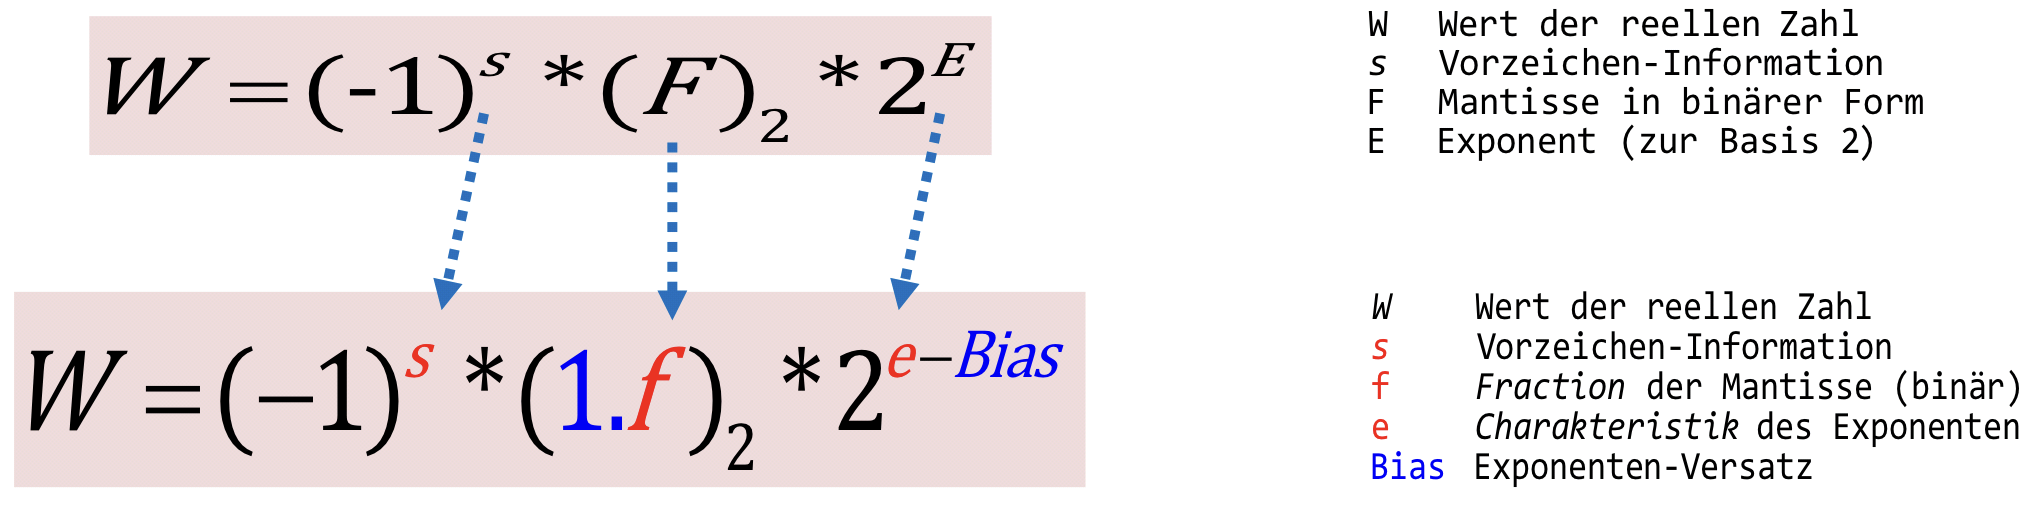
\includegraphics[width=12cm]{pics/IEEE-Grundformat_Darstellung}\\
	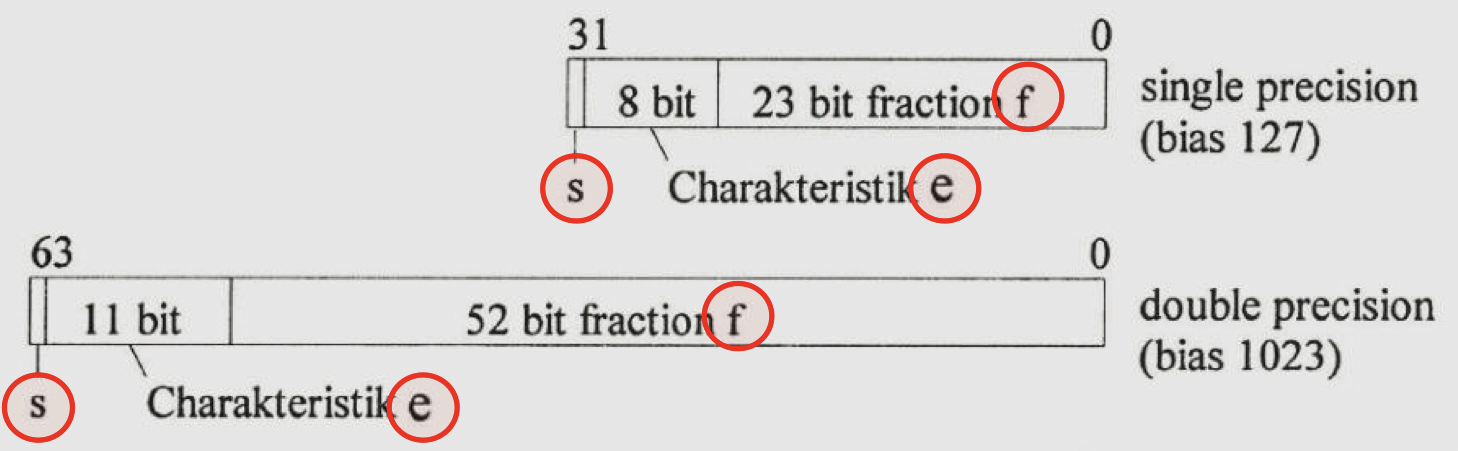
\includegraphics[width=9cm]{pics/IEEE-Grundformat}\\

\begin{minipage}[t]{9cm}
	\subsubsection{IEEE 754: Charakteristik}
	Die Exponenten-Information \color{red} \textbf{e} \color{black} wird auch als \textbf{Charakteristik} bezeichnet. Der transformierte Exponent \color{red} \textbf{e} \color{black} ergibt sich durch das Erh"ohen des Exponenten \textbf{E} um einen definierten \textbf{Bias} (Darstellung im \textbf{Excess-Code}).\\
	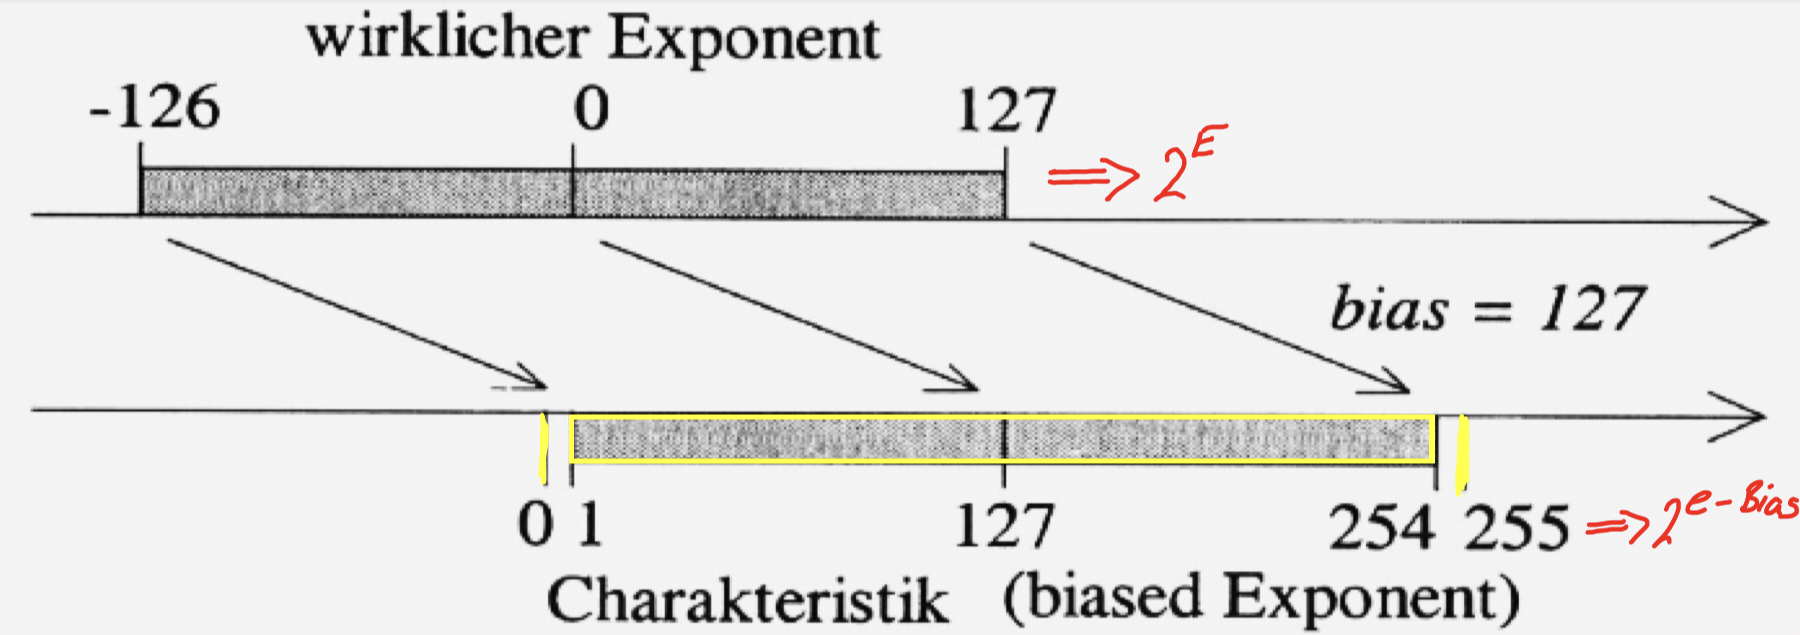
\includegraphics[width=7cm]{pics/IEEE-Exponent}
	\vspace{2ex}
	\subsubsection{Wertebereich und Kenngr"ossen}
	Kennwerte und Wertebereich f"ur die normalisierte Darstellung.\\
	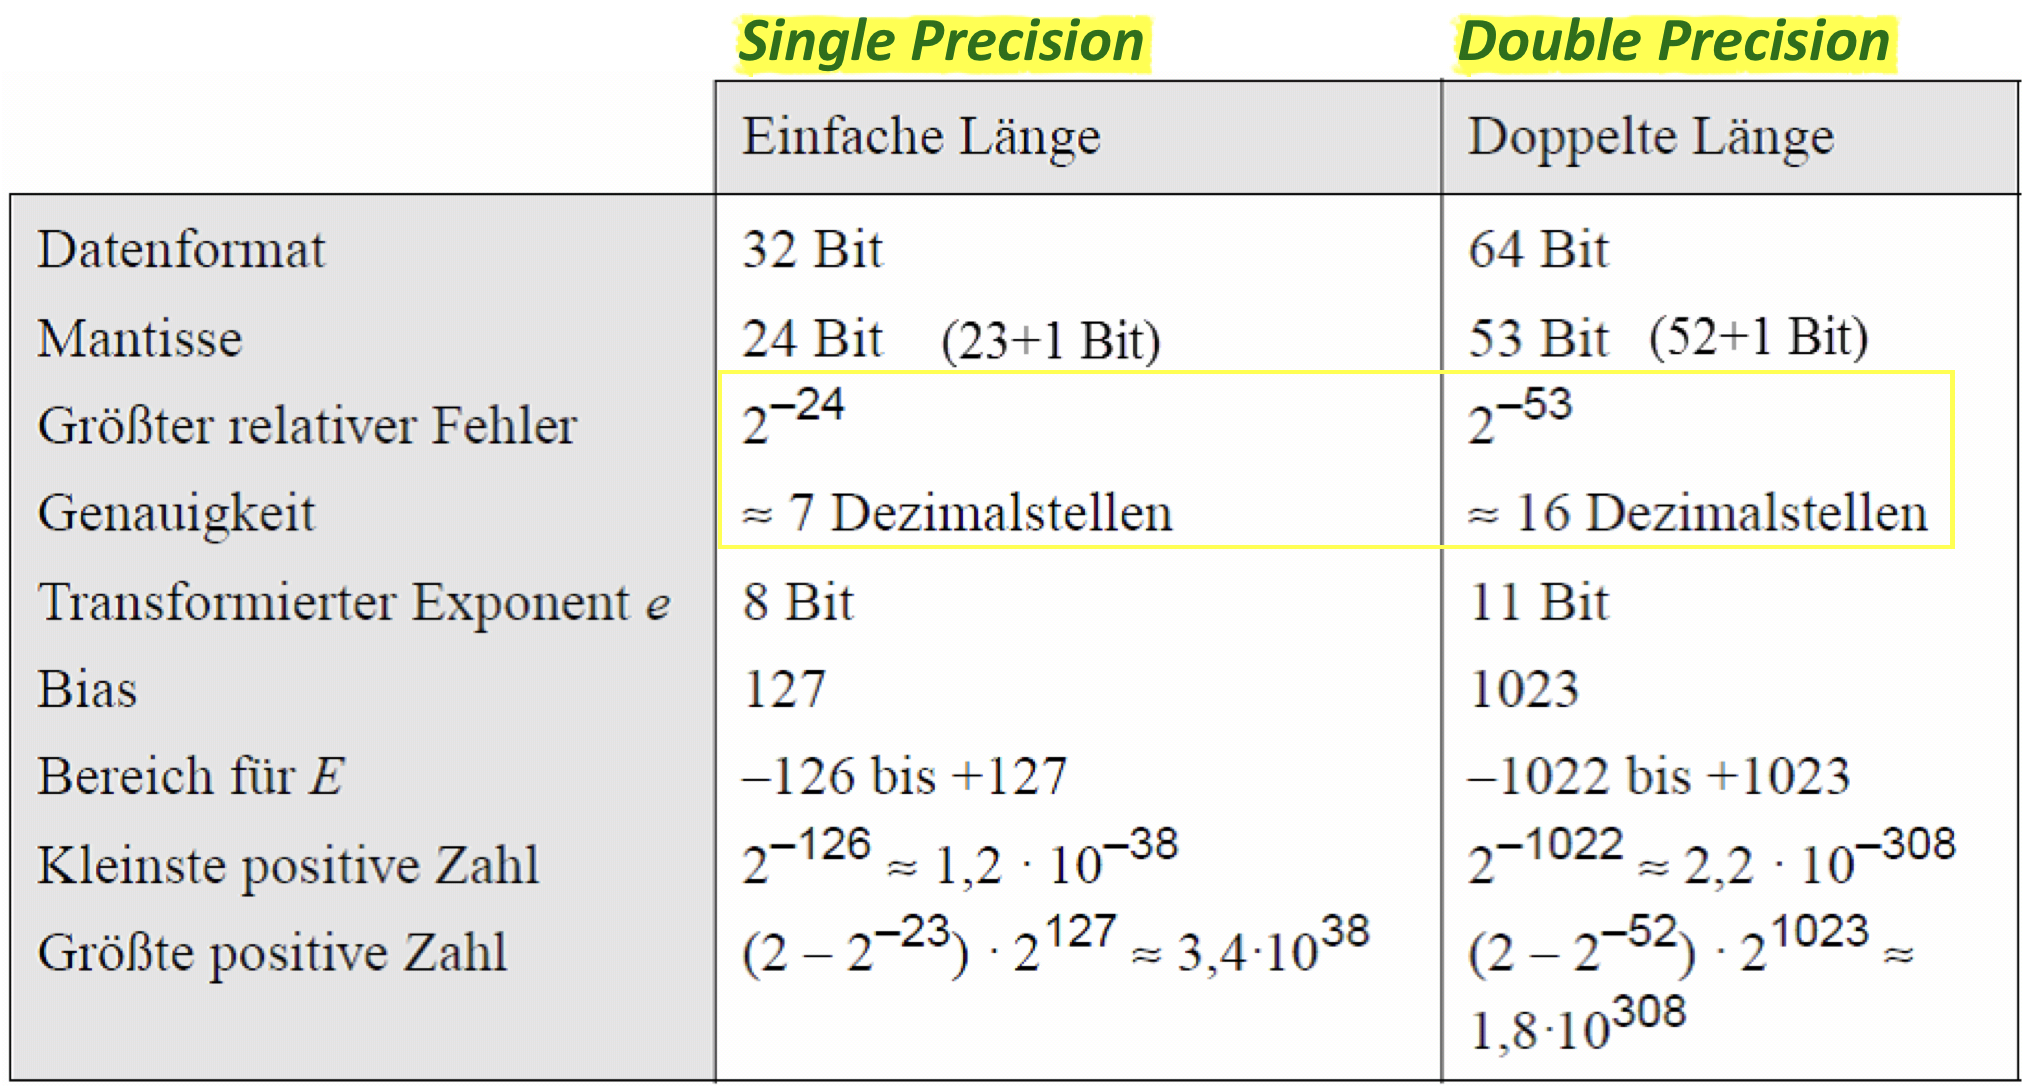
\includegraphics[width=8cm]{pics/IEEE-Wertbereich}
	\vspace{2ex}
	\subsubsection{IEEE 754: Berechnungsformeln}
		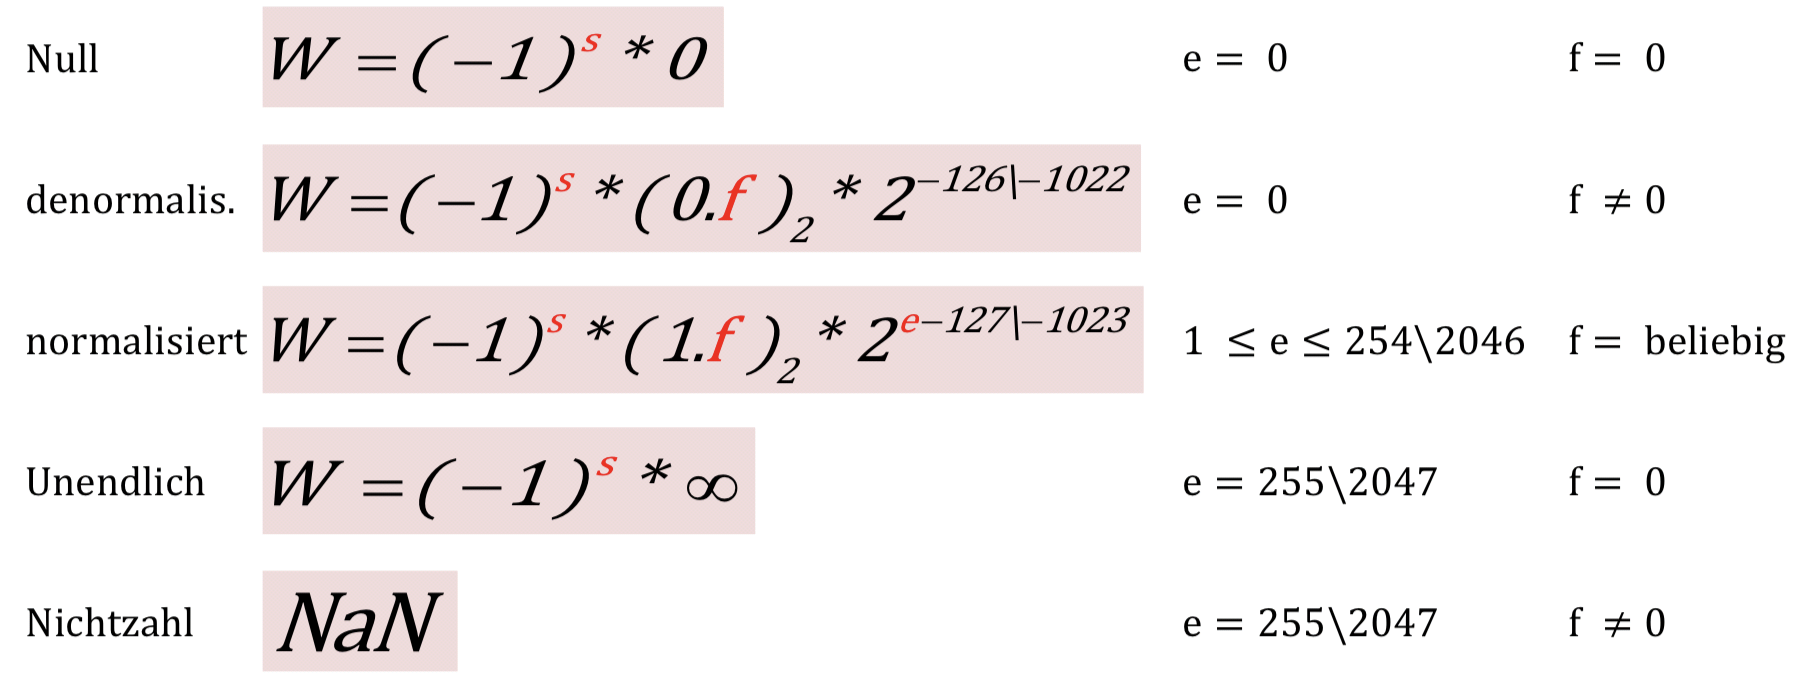
\includegraphics[width = 10cm]{pics/IEEE-Berechnungsformel}

\end{minipage}
%
\begin{minipage}{0.5cm}
	\ \
\end{minipage}
%
\begin{minipage}[t]{9cm}
			
	\subsubsection{Floating Point Operationen}
		\begin{tabbing}
			\textbf{Add}\=\textbf{ition, Subtraktion}\\
			\> Wenn die Exponenten ungleich sind muss der kleiner\\ 
			\> am gr"osseren angepasst werden. Dann werden die\\ 
			\> Mantissen addiert und wenn n"otig muss das Resultat\\ 
			\> noch normalisiert werden.\\
	
			\textbf{Multiplikation, Division}\\
			\> Bei der Multiplikation oder Division m"ussen die\\
			\> Exponenten addiert oder subtrahiert werden und die\\ 
			\> Mantissen mit der jeweiligen Operation verrechnet\\ 
			\> werden.
		\end{tabbing}

	\subsubsection{Zahlengerade f"ur Single Precision Numbers}
		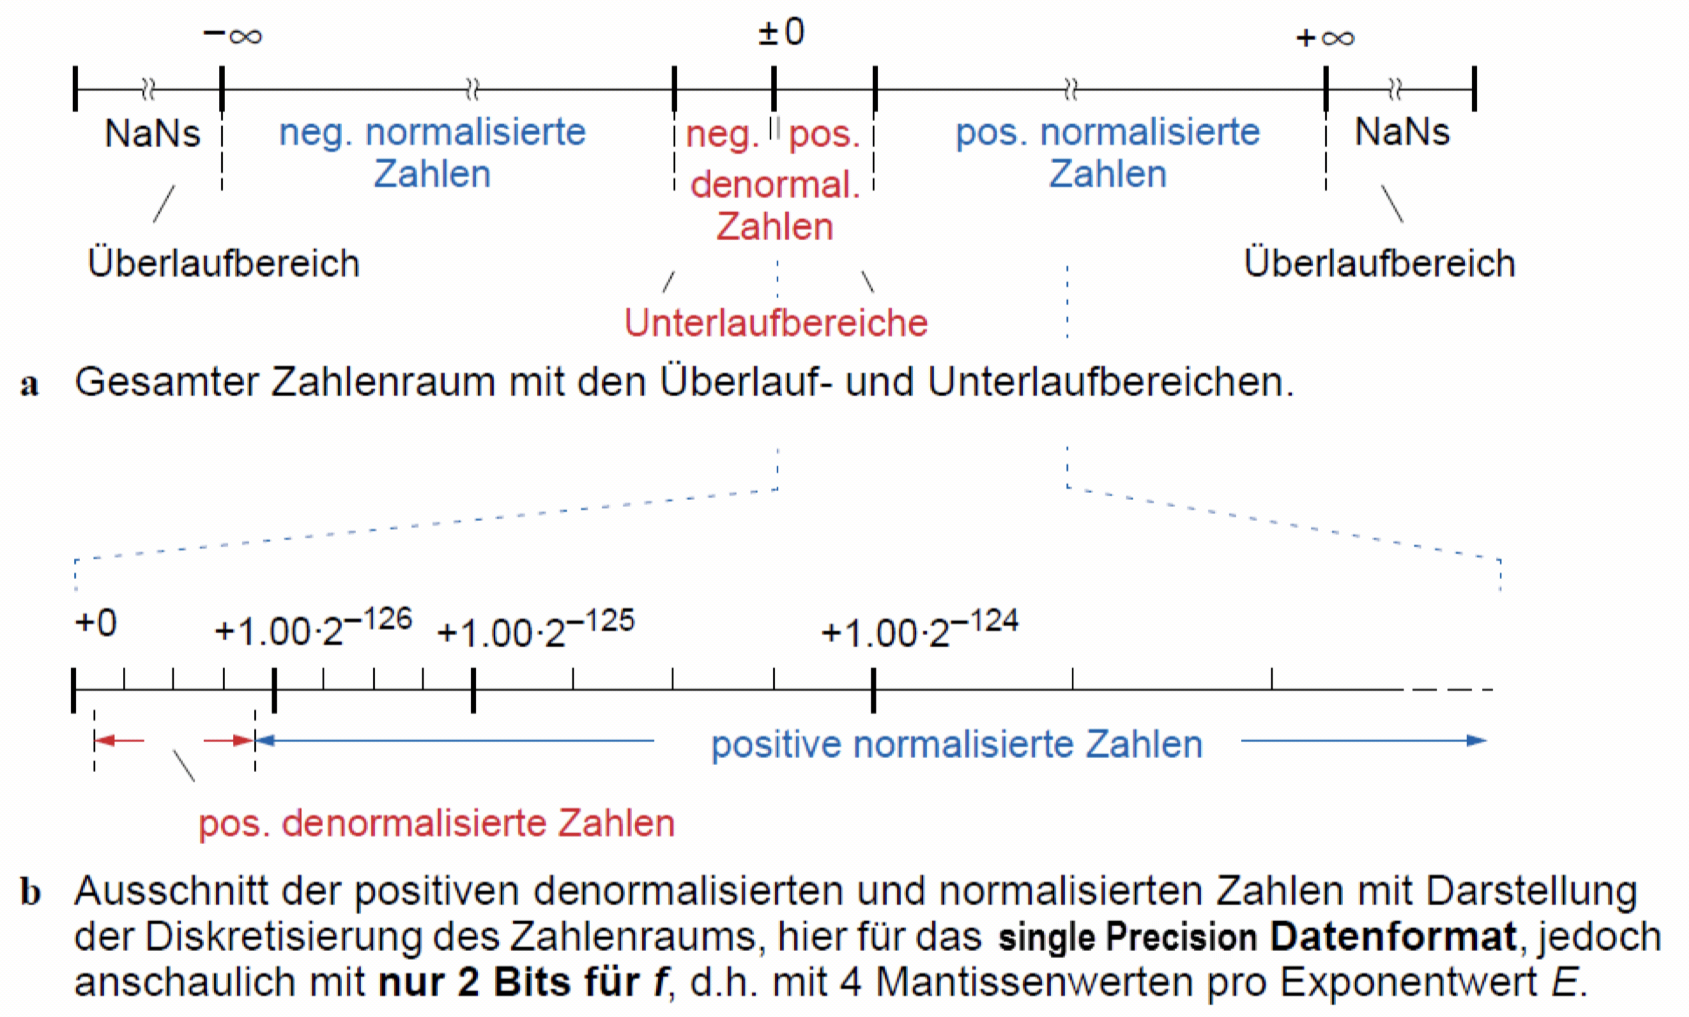
\includegraphics[width=9cm]{pics/IEEE-Zahlengerade}

\end{minipage}

\subsection{Zahlencodes}
Ein Code ist eine Vorschrift f"ur die eindeutige Zuordnung (Codierung) zweier Zeichenmengen (Urmenge, Bildmenge).
Folgende Numerische Codes sind von Bedeutung:
\begin{itemize}
	\item Zifferncodes: Jede Ziffer wird getrennt codiert, z.B. BCD.
	\item Positionscodes: Position des Bits innerhalb eines Wortes von Bedeutung
	\item Bewertbare Codes: Bitposition i hat definierte Wertigkeit, z.B. 8-4-2-1-Code
	\item Anordnungscodes: definiertes Bildungsgesetz, z.B. Excess-Code
	\item Einschrittige Codes: haben konstante Hamming-Distanz von 1
	\item Gleichgewichtete Codes (m-aus-n Codes): enthalten bei n Ziffernstellen m Einsen
	\item Fehlererkennungscodes: z.B. Dual-Code mit Parit"atsbit
	\item Fehlerkorrektur-Codes: erm"oglichen die Erkennung und die Korrektur falscher Bits
\end{itemize}

\subsubsection{BCD-Code}
\begin{minipage}{9cm}
\vspace{-8ex}
	Bei der BCD-Codierung (\textbf{Binary Coded Decimals}) werden die Ziffern der Dezimalzahl separat mit je vier Bit codiert. Der BCD-Code wird haupts"achlich verwendet um Rundungsfehler vermeiden zu k"onnen und Werte exakt darstellen zu k"onnen.\\
	Die sechs nicht verwendeten Bin"arwerte nennt man \textbf{Pseudotetraden}.
	\vspace{2ex}

	Beim Rechnen mit BCD-Zahlen muss auf Pseudotetraden geachtet werden, wenn solche entstehen m"ussen diese mit einer zus"atzlichen Addition von +6 korrigiert werden.
	\vspace{2ex}
	
	Beim Speichern von BCD-Zahlen gibt es das Packed- und Unpacked-BCD-Format. Beim \textbf{Unpacked BCD} wird jede BCD-Ziffern in der kleinsten adressierbaren Speichereinheit abgelegt. Beim \textbf{Packed BCD} werden mehrere BCD-Ziffern in eine Speichereinheit $"$gepackt$"$.
\end{minipage}
%
\begin{minipage}{0.5cm}
	\ \
\end{minipage}
%
\begin{minipage}{9cm}
	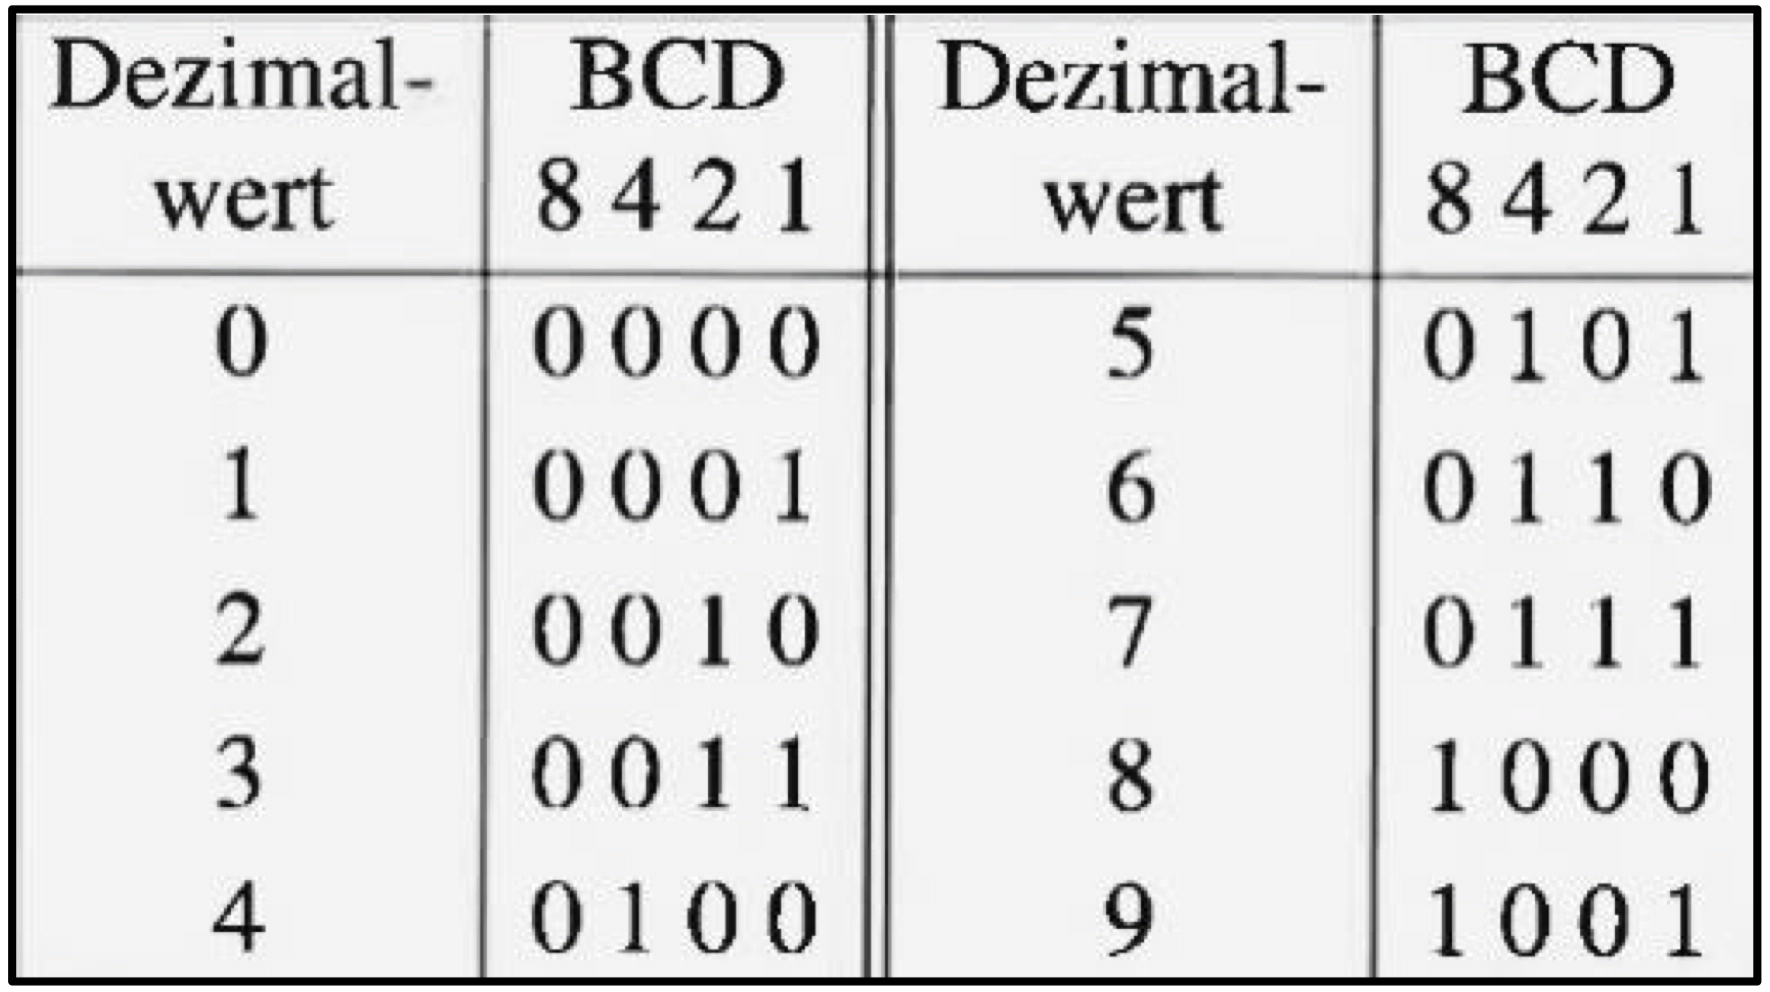
\includegraphics[width=4.5cm]{pics/2-BCD-Code}\\
	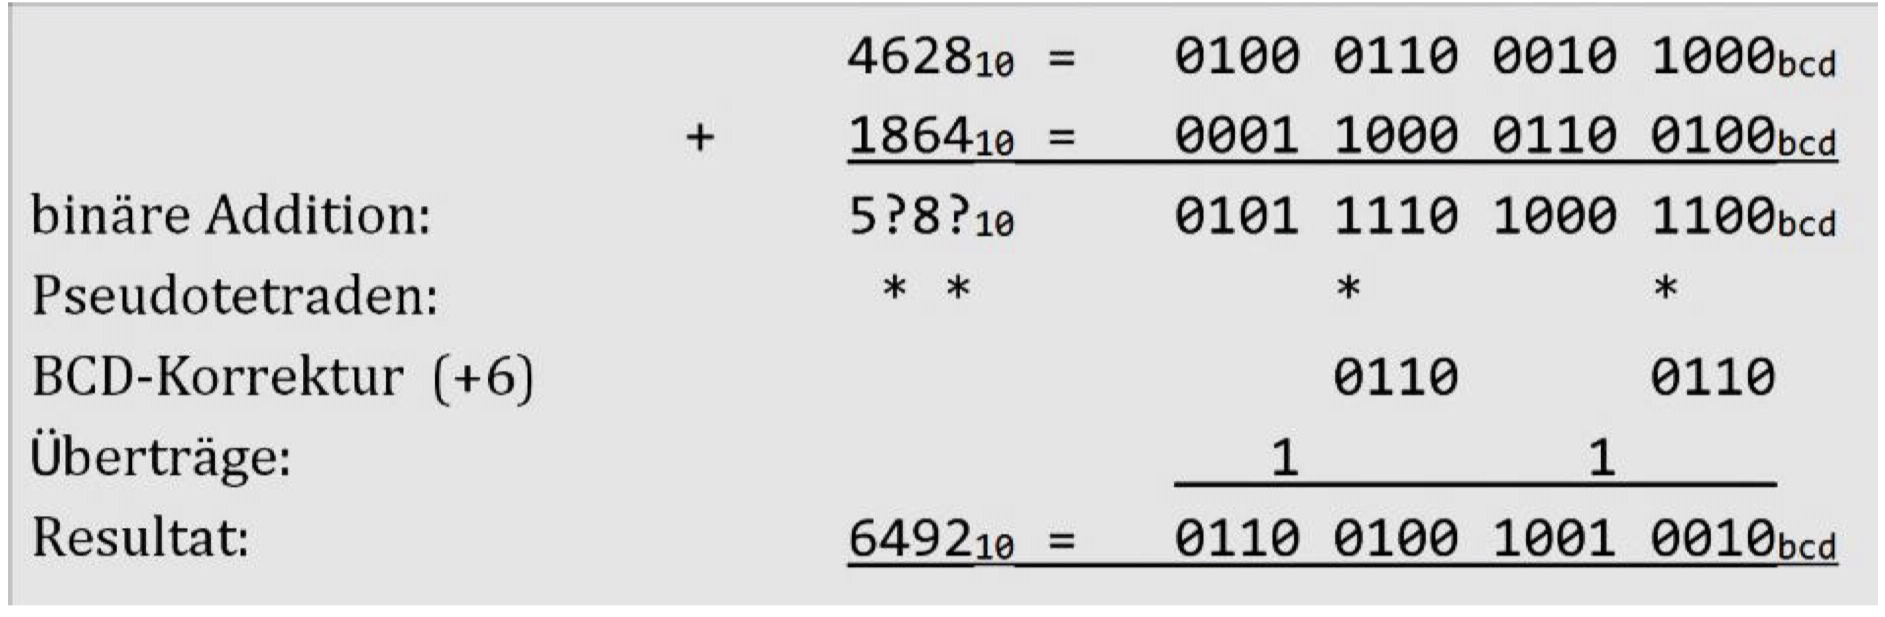
\includegraphics[width=8cm]{pics/2-Pseudo_Tetrade}\\
	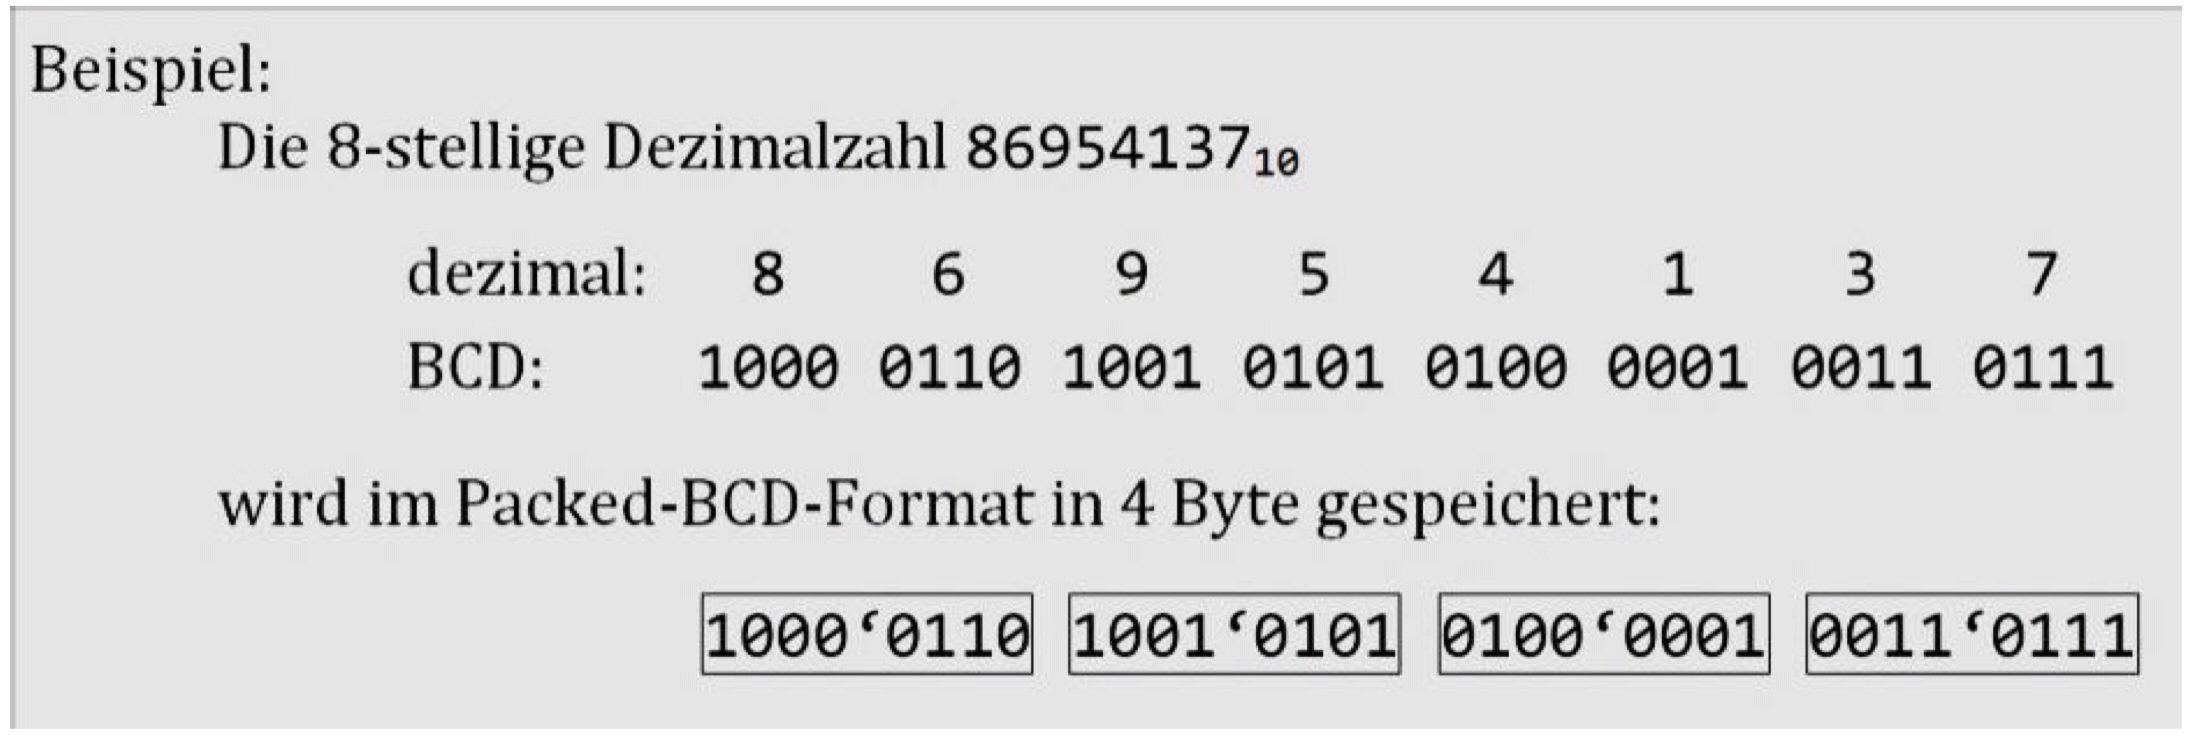
\includegraphics[width=8cm]{pics/2-Packed-BCD}
\end{minipage}

\subsubsection{Z"ahlcodes}
\begin{minipage}{9cm}
	\vspace{-6ex}
	Der Z"ahlcode kann sehr einfach codiert und decodiert werden und wird bei der Telefonimpulswahl verwendet: Die Einsen werden als Impulse umgesetzt, die Nullen als $"$keine Impulse$"$.
\end{minipage}
%
\begin{minipage}{0.5cm}
	\ \
\end{minipage}
%
\begin{minipage}{9cm}
	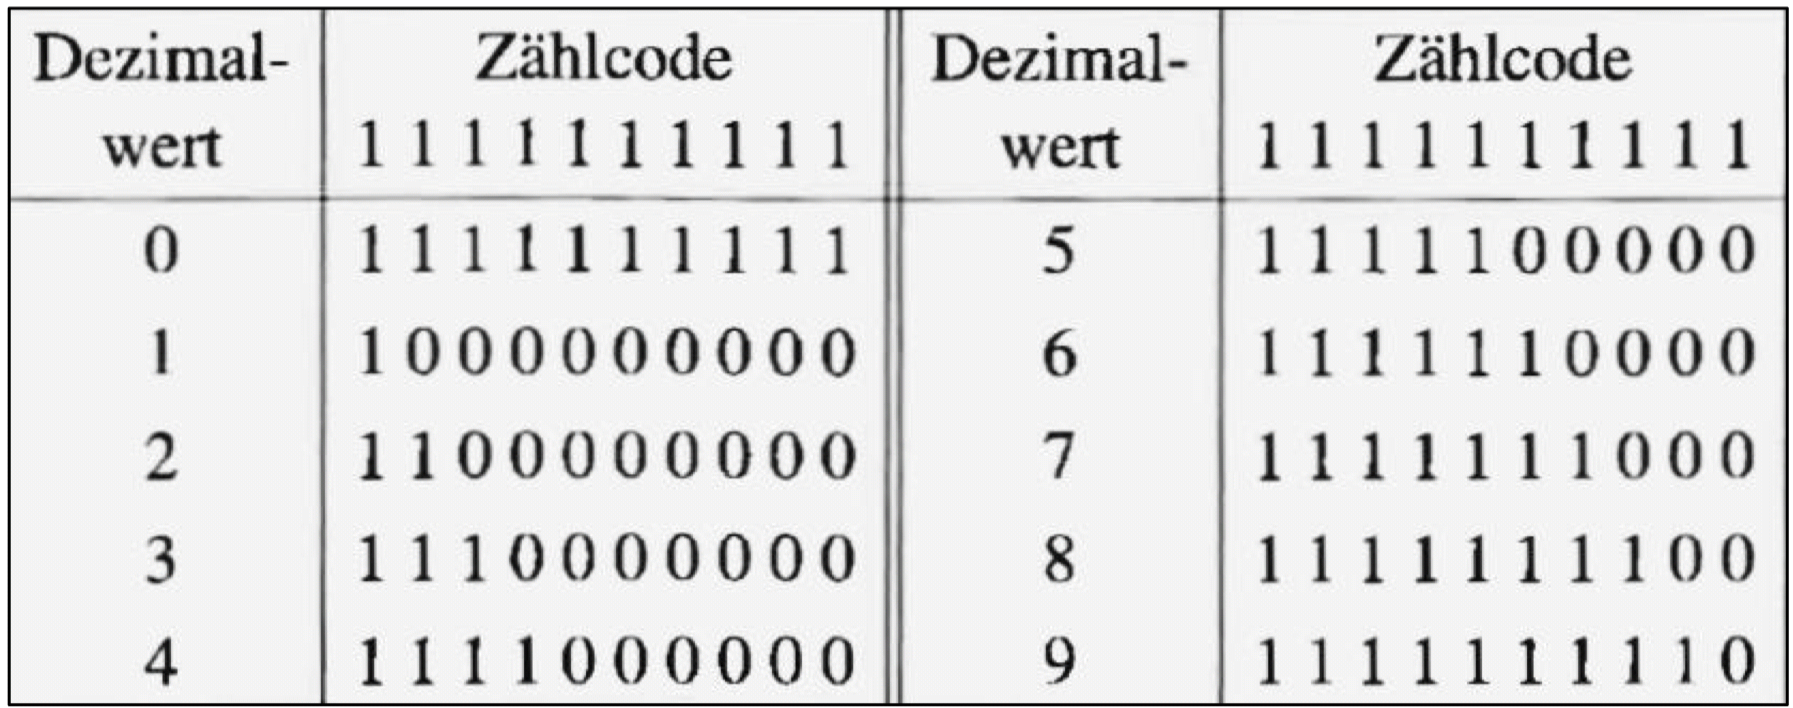
\includegraphics[width=6cm]{pics/2-Zaehlcodes}
\end{minipage}

\subsubsection{Codes mit Fehlererkennung}
Aus Gr"unden der Fehlererkennung werden oft \textbf{gleichgewichtete m-aus-n Codes} verwendet: z.B. in der Telekommunikation oder bei den Strichcodes.

\subsubsection{Gray-Code}
\begin{minipage}{9cm}
\vspace{-12ex}
	Der Gray-Code ist eine andere Darstellungsform des Bin"arcodes. Er hat die Eigenschaft, dass beim fortlaufenden Z"ahlen zwischen zwei benachbarten Codew"ortern immer nur ein Bit den Zustand wechselt (\textbf{einschrittiger Code}). Damit ergeben Ablesefehler im Zwischenbereich jeweils nur eine Unsicherheit von einem Bit, was gerade der Aufl"osegenauigkeit der gew"ahlten Codierung entspricht.
\end{minipage}
%
\begin{minipage}{0.5cm}
	\ \
\end{minipage}
%
\begin{minipage}{9cm}
	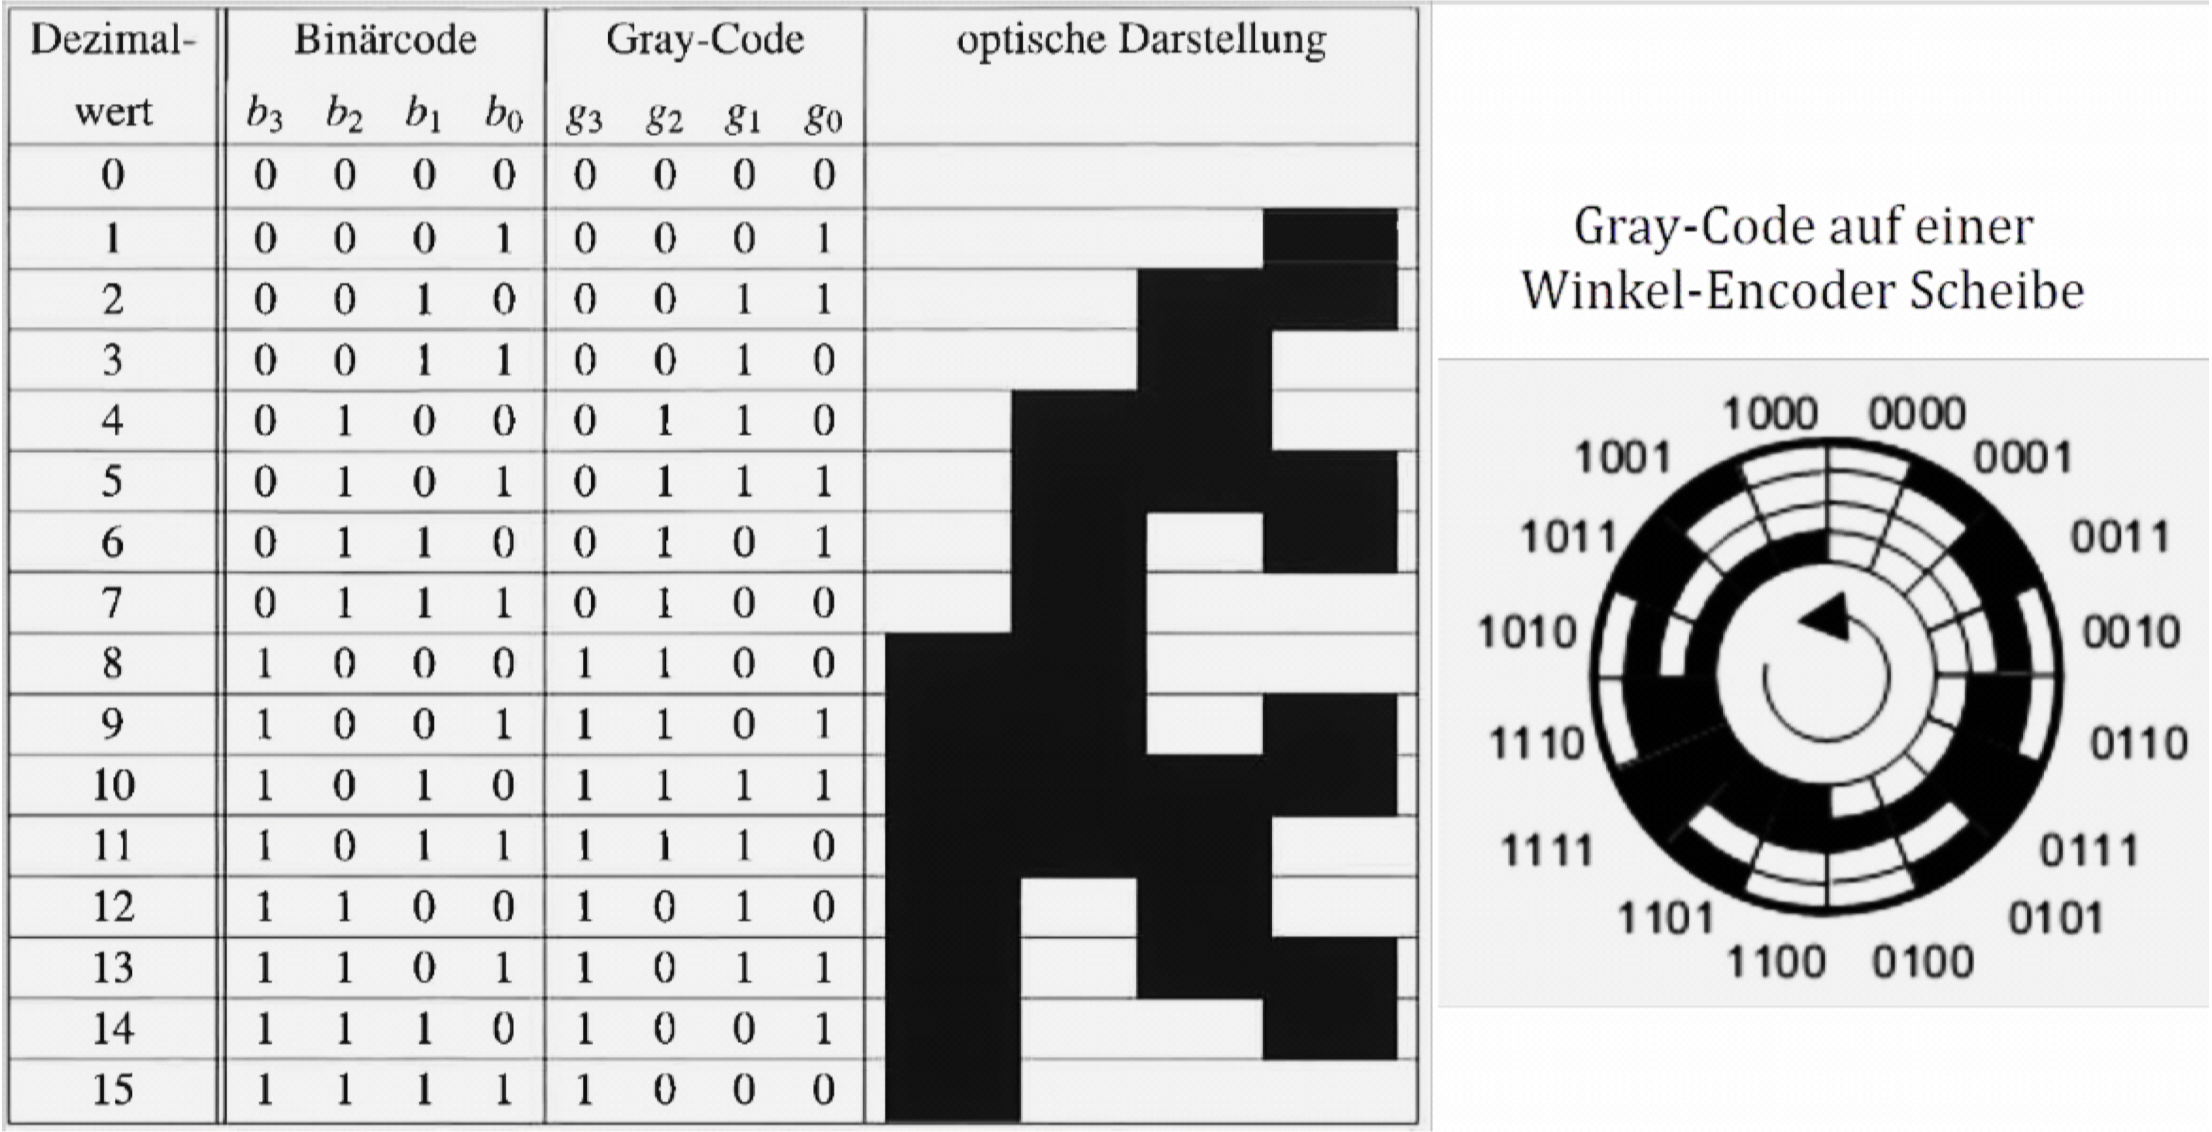
\includegraphics[width=9cm]{pics/2-Gray-Code}
\end{minipage}

\subsection{Zeichencodes}
\textbf{Alphanumerische Codes} dienen zur Darstellung von Ziffern, Buchstaben und  Sonderzeichen. Der am weitaus verbreiteste Zeichencode ist der \textbf{ASCII-Code}

\subsubsection{Unicode: universelle 16- und 32-Bit-Codes}
\begin{minipage}{9cm}
\vspace{-4ex}
	Der 16-Bit-Zeichencode UCS-2 wurde 1992 vom IEC genormt: Er enth"alt systematisch alle wichtigen nationalen und internationalen Zeichens"atze und den ASCII-Code als Untermenge am Anfang der Tabelle ab Index 0x0000.\\
	
	Dieser 16-Bit-Zeichencode ist wiederum eine Untermenge des 32-bit-Codes UCS-4, welcher Platz f"ur total 2 Milliarden Zeichen bietet.
\end{minipage}
%
\begin{minipage}{0.5cm}
	\ \
\end{minipage}
%
\begin{minipage}{9cm}
	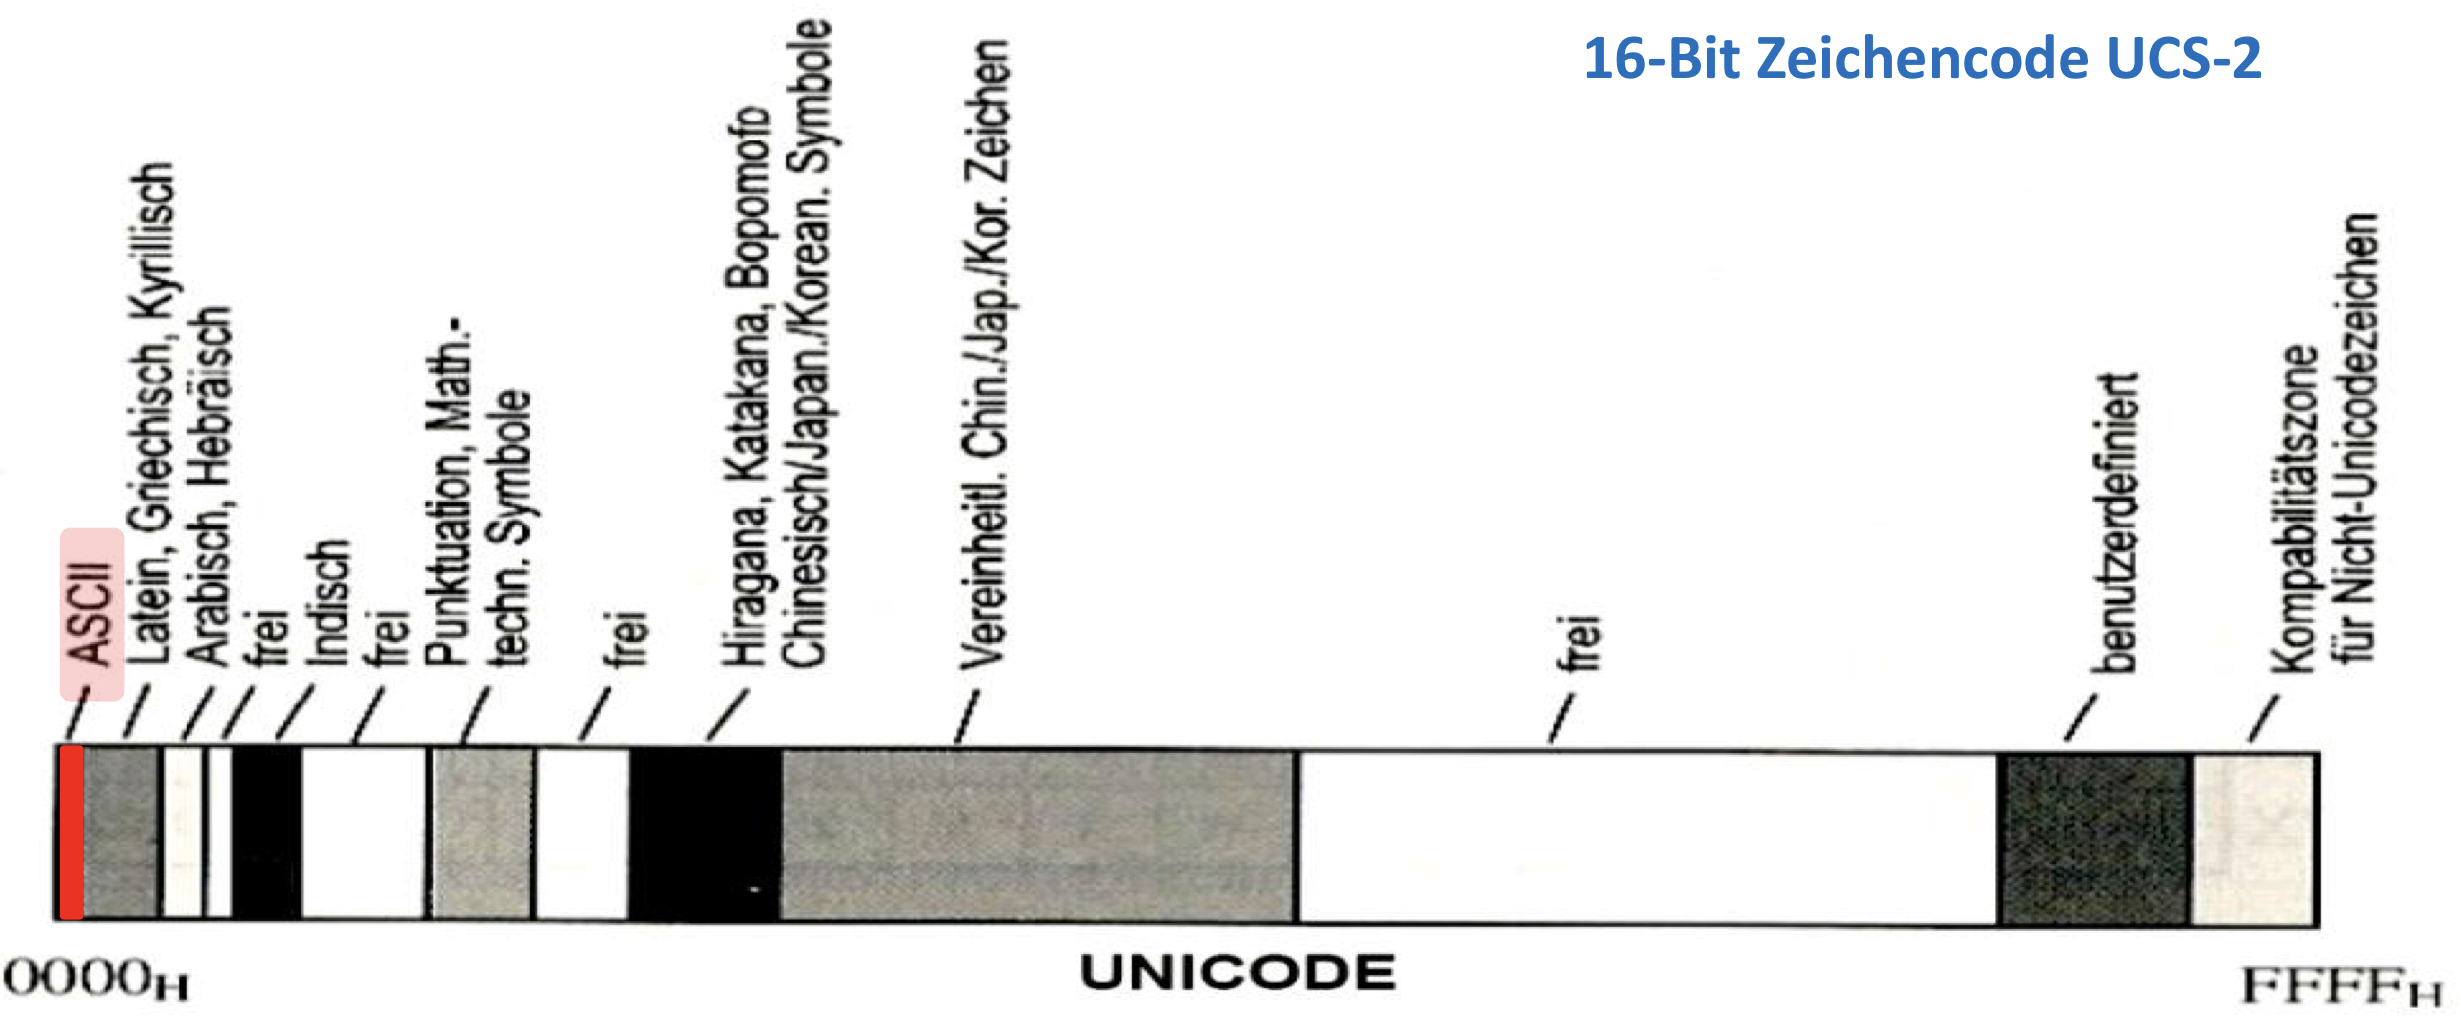
\includegraphics[width=9cm]{pics/2-Unicode}
\end{minipage}

\subsection{Fehlererkennung}
Aufgrund der Informationstheorie k"onnen Aussagen "uber die zus"atzlich notwendige Redundanz gemacht werden, um Ein- und Mehrbitfehler zu erkennen und allenfalls zu korrigieren.\\
Um eine Fehlererkennung durchf"uhren zu k"onnen ben"otigt es einen Codier-Mehraufwand (Redundanz). Solange alle Code-Kombinationen g"ultige Codeworte sind, wirkt sich jeder Fehler so aus, dass wiederum ein g"ultiges Codewort entsteht.

\vspace{2ex}
\begin{minipage}{9cm}
	\subsubsection{Definition}
		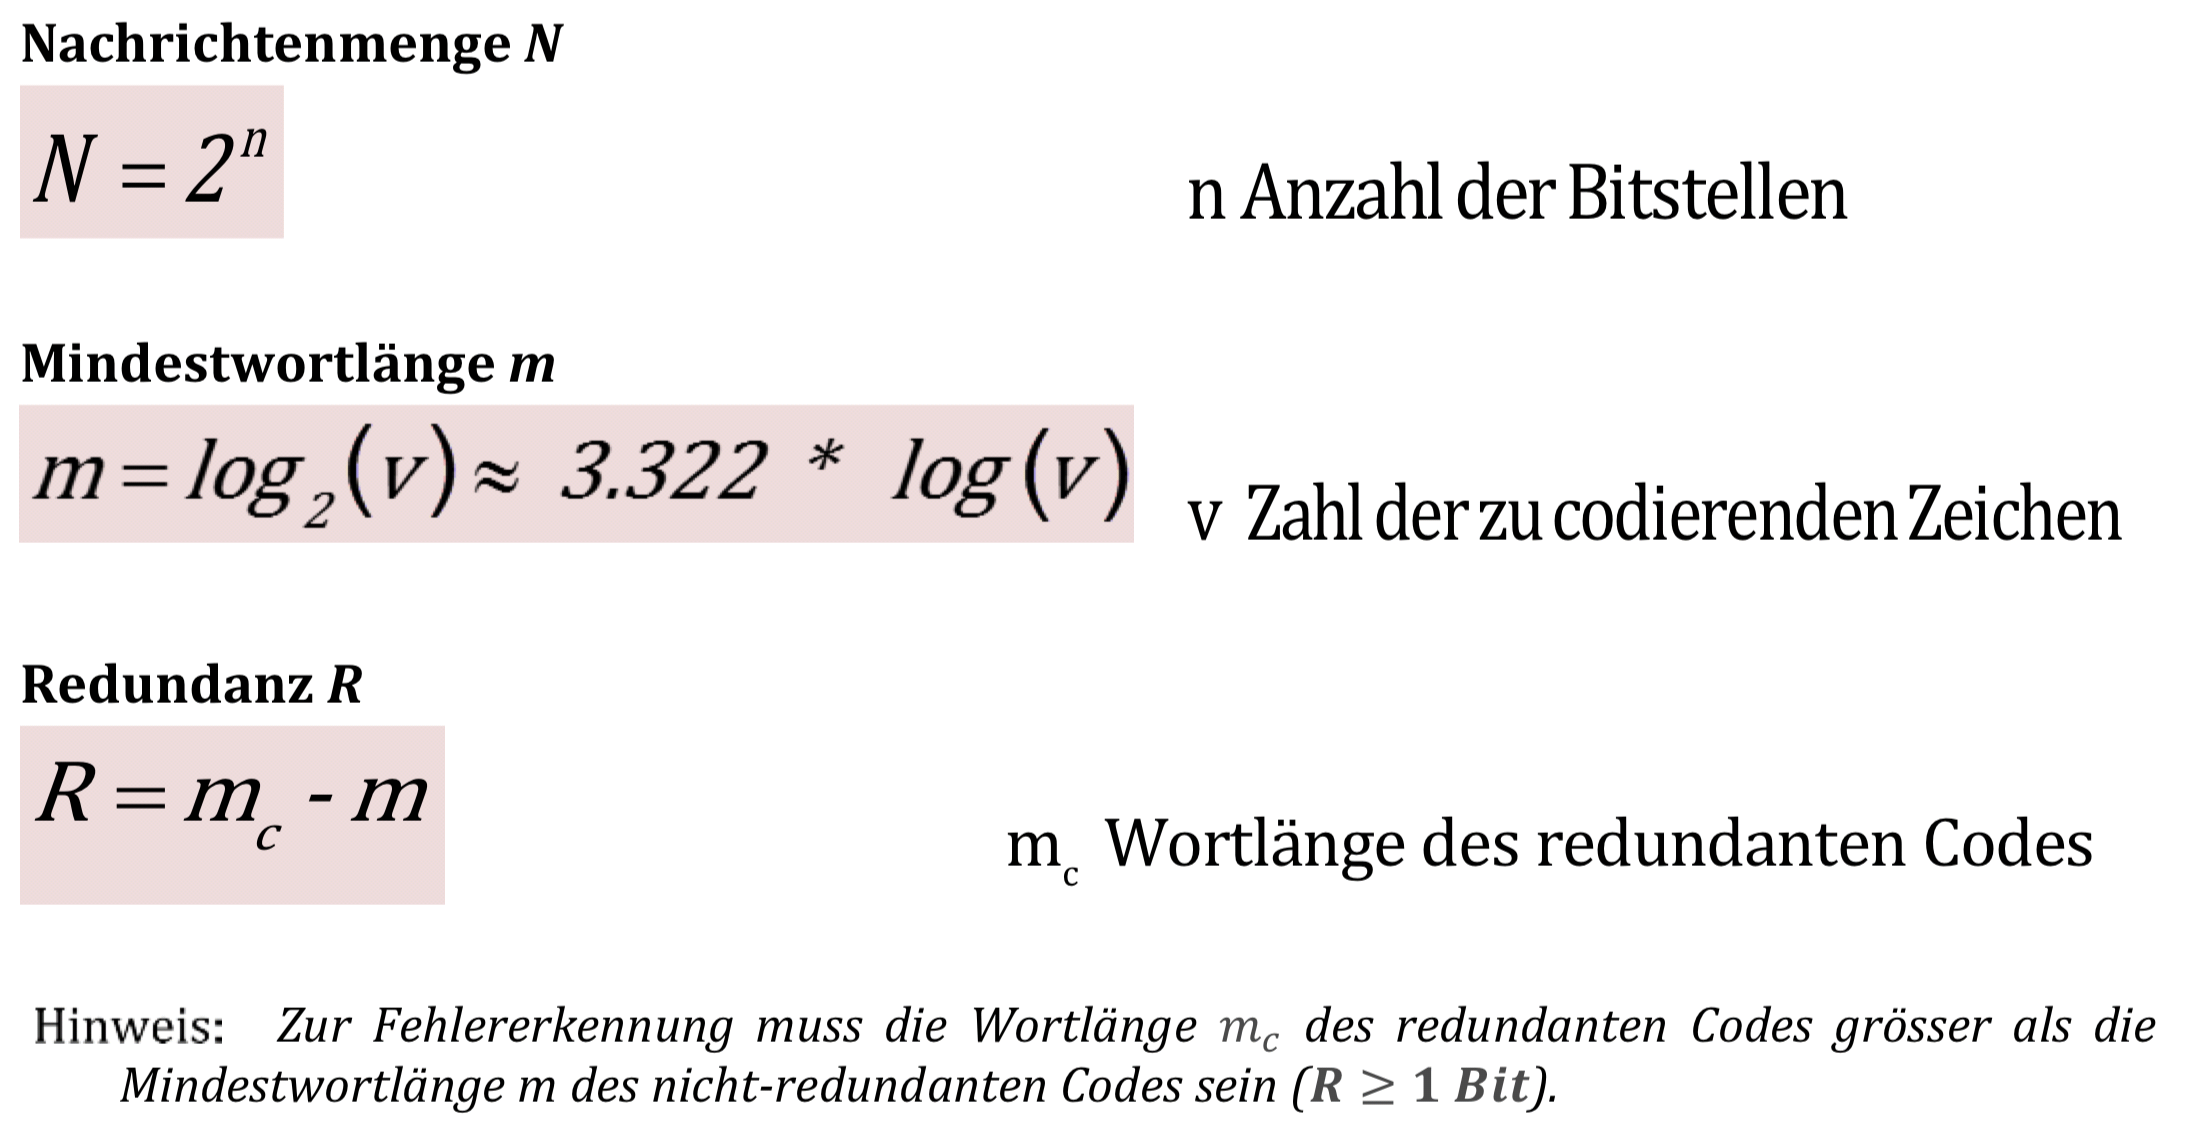
\includegraphics[width=9cm]{pics/2-Fehlererkennung1}\\
		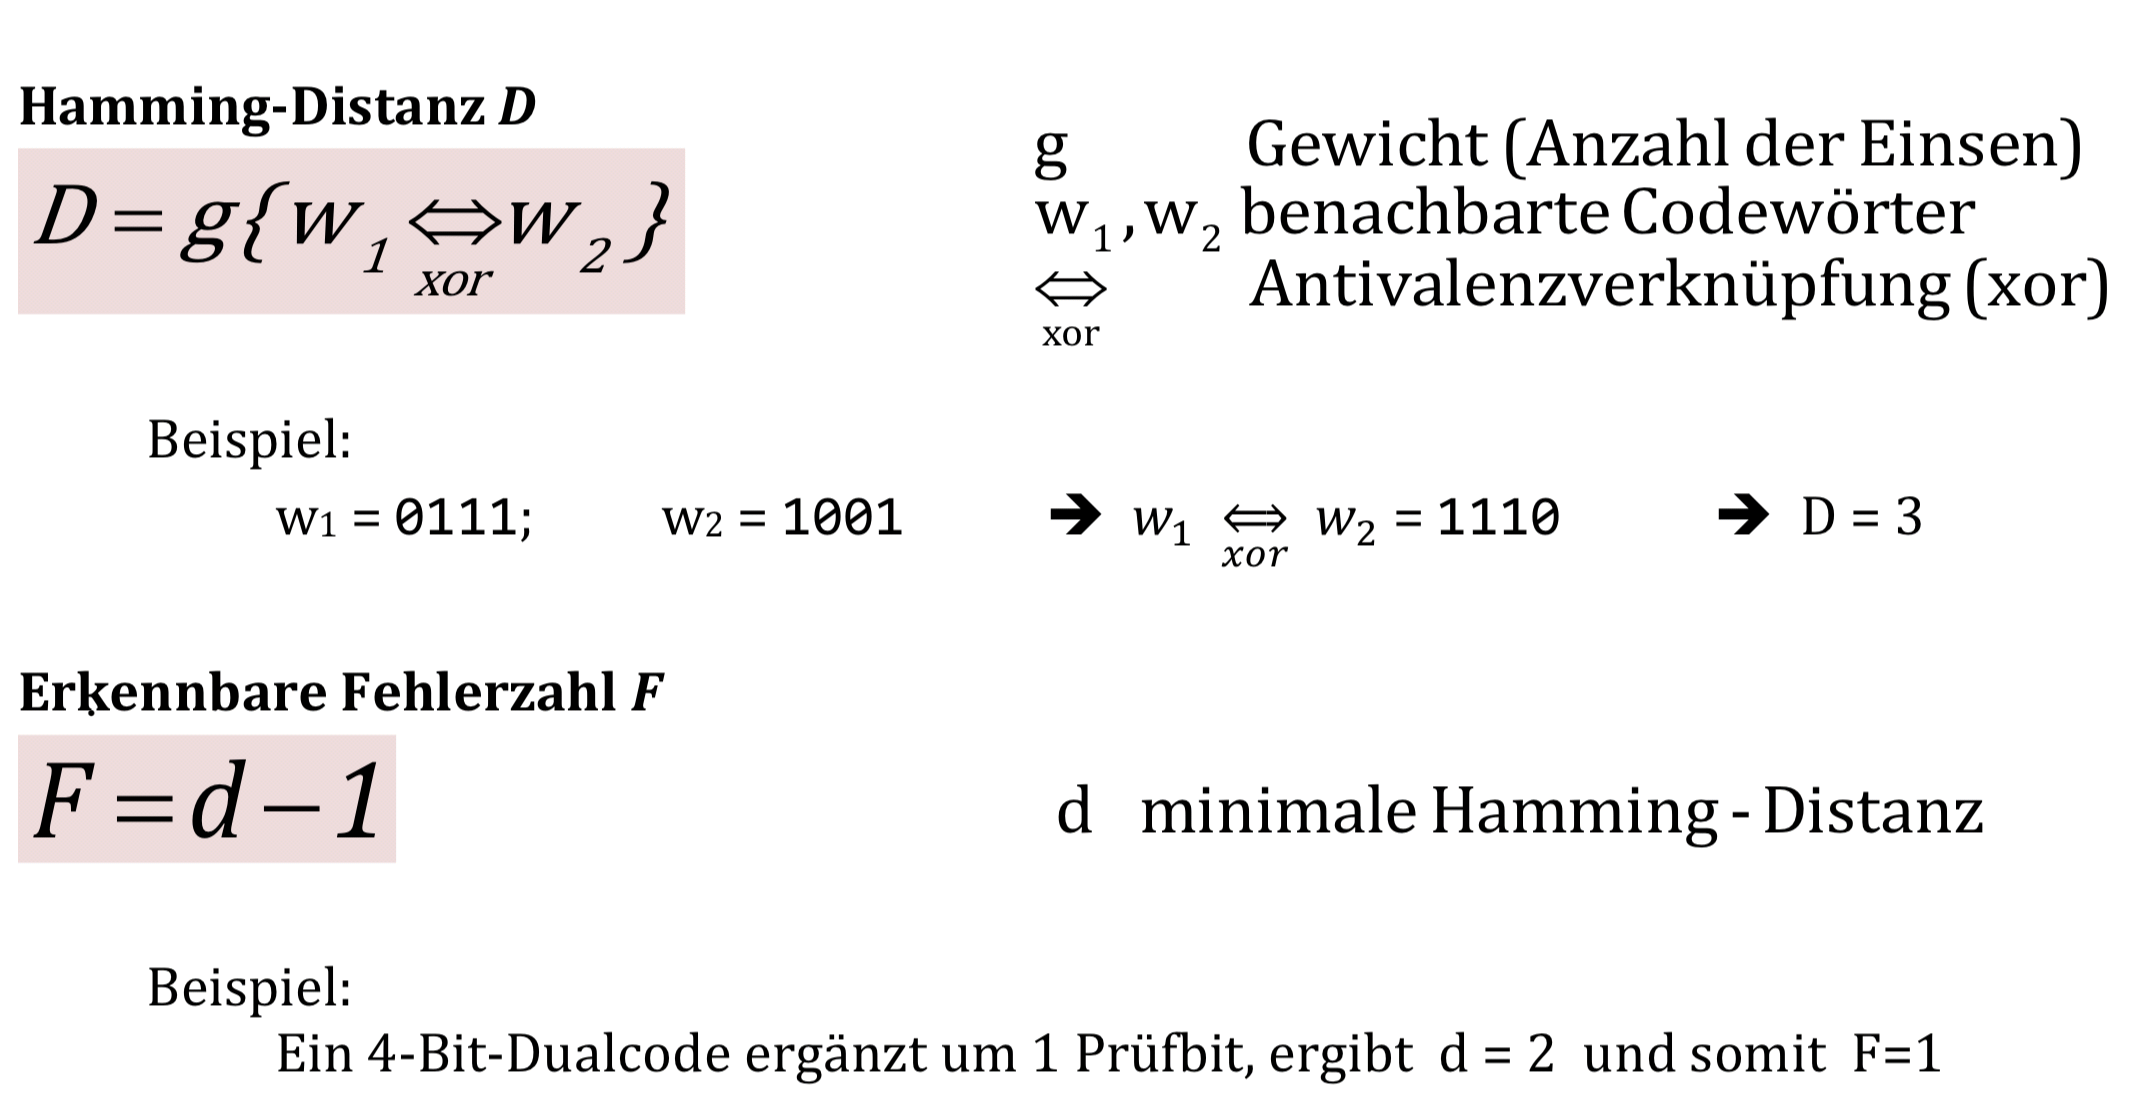
\includegraphics[width=9cm]{pics/2-Fehlererkennung2}
\end{minipage}
%
\begin{minipage}{0.5cm}
	\ \
\end{minipage}
%
\begin{minipage}{9cm}
	\subsubsection{Parity}
		Die in der Computer- und "Ubertragungstechnik weitverbreiteste und bekannteste Fehlererkennungsmethode ist das Parit"atsbit. Ein zus"atzliches Bit wird bei jedem g"ultigen Codewort z.B. auf eine gerade Parit"at erg"anzt. Damit wird jeder Einbit-Fehler an
			der ungeraden Summe von Einsen leicht erkennbar. Alle 
			g"ultigen Codeworte (inklusive Parit"atsbit) unterscheiden sich voneinander an mindestens zwei Stellen (Hamming-Distanz D=2).\\ 
			
	\begin{minipage}{6cm}
		\textbf{Definition Even und Odd Parity:}\\
		Das Parity-Bit wird in die $"$Z"ahlung der Einsen$"$ miteinbezogen, d.h. bei \textbf{Even Parity} wird das Parit"atsbit so gesetzt, dass die Anzahl Einsen inklusive Parity-Bit gerade ist: Eine ungerade Anzahl Einsen in einem Datenwort f"uhrt also zu einem Parity-Bit =1; damit
			wird die gesamte Anzahl Einsen gerade.\\
			 \textbf{Odd Parity} bedeutet: 
			Das Datenwort inklusive Parity-Bit besitzt eine ungerade 
			Anzahl Einsen.
	\end{minipage}
	%
	\begin{minipage}{0.2cm}
		\ \
	\end{minipage}
	%
	\begin{minipage}{2.6cm}
		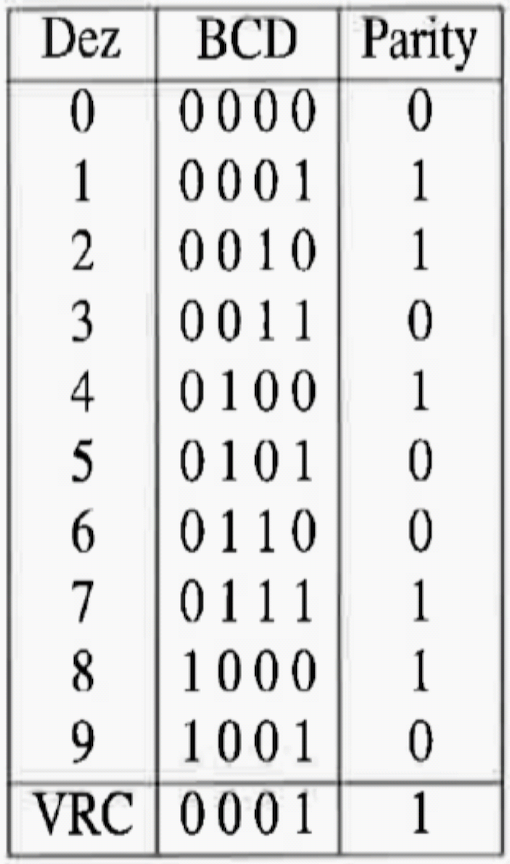
\includegraphics[width=2.6cm]{pics/2-Parity}\\
		\begin{small}
			\textit{Bsp. Even-Parity}
		\end{small}
	\end{minipage}
\end{minipage}

\subsubsection{CRC}
	\begin{minipage}{9cm}
		Das Problem der einfachen Parit"atspr"ufung besteht in ihrer Anf"alligkeit auf Mehrbitfehler: Sobald in einem mit Parity gesicherten Wort nicht nur ein, sondern zwei Bits gest"ort sind, kann dieser Fehler nicht erkannt werden. Die Fehlererkennungsrate bei einfacher Parity betr"agt nur 50\%, da alle geradzahligen Fehler nicht erkannt werden k"onnen.\\

		Mit der CRC-Technik (\textbf{Cyclic Redundancy Check}) k"onnen mit relativ wenig Aufwand Mehrfach- und Burst-Fehler (mehrere Fehler kurz hintereinander) in Datenbl"ocken entdeckt werden. Die CRC-Technik wird heute sehr verbreitet in der Datenspeicherung
			und der Daten"ubertragung (Computernetzwerke) angewendet.\\
	\end{minipage}
	%
	\begin{minipage}{0.5cm}
		\ \
	\end{minipage}
	%
	\begin{minipage}{9cm}
		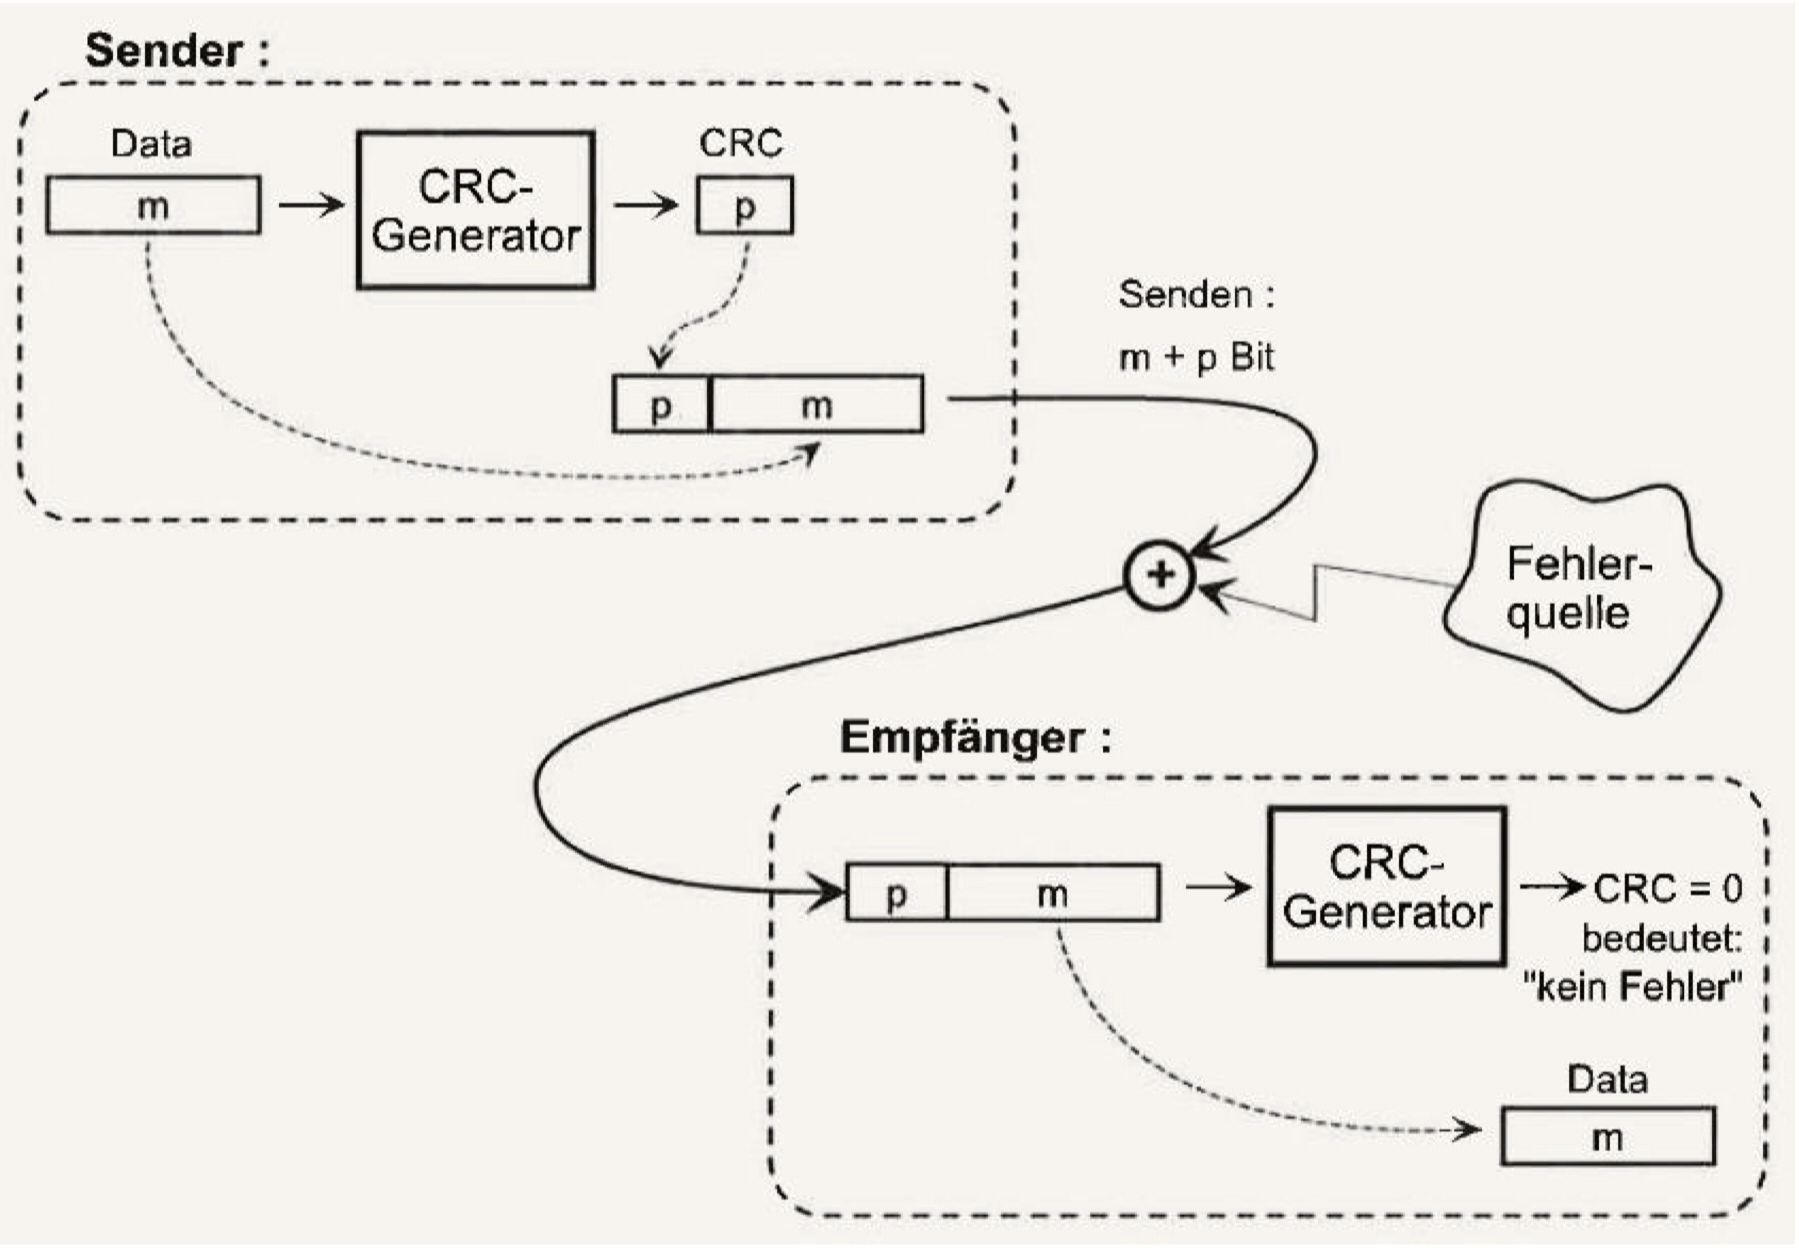
\includegraphics[width=8cm]{pics/2-CRC-Generator}
	\end{minipage}
	
	
\newpage
